
% !TEX encoding = UTF-8 Unicode



\documentclass[a4paper]{article}
\usepackage{dirtytalk}
\usepackage{geometry}
\geometry{
  a4paper,
    total={150mm,247mm},
    left=30mm,
    top=30mm,
}
\usepackage{quotchap}
\usepackage{pgfplotstable,filecontents}
\pgfplotsset{compat=1.9}% supress warning
\usepackage{graphicx}
\usepackage{epstopdf}
\DeclareGraphicsExtensions{.eps}
\usepackage{url}
\usepackage{multicol}% http://ctan.org/pkg/multicols
\usepackage{epigraph}
\setlength{\epigraphwidth}{.85\textwidth}

\usepackage[utf8x]{inputenc} 

\usepackage{array}
\newcolumntype{L}[1]{>{\raggedright\let\newline\\\arraybackslash\hspace{0pt}}m{#1}}
\newcolumntype{C}[1]{>{\centering\let\newline\\\arraybackslash\hspace{0pt}}m{#1}}
\newcolumntype{R}[1]{>{\raggedleft\let\newline\\\arraybackslash\hspace{0pt}}m{#1}}
\usepackage{subcaption}
\usepackage[utf8]{inputenc}
\usepackage[portuguese]{babel}
\usepackage{listings,mdframed}

\usepackage{textcomp}
\usepackage{hyperref}

\usepackage{float}
\usepackage{listings}

\lstdefinestyle{esc} {
  language=c,
    keywordstyle=\bfseries\ttfamily\color[rgb]{0,0,1},
    identifierstyle=\ttfamily,
    commentstyle=\color[rgb]{0.133,0.545,0.133},
    stringstyle=\ttfamily\color[rgb]{0.627,0.126,0.941},
    showstringspaces=false,
    basicstyle=\tiny,
    numberstyle=\small,
    numbers=right,
    stepnumber=1,
    numbersep=10pt,
    tabsize=1,
    breaklines=true,
    prebreak = \raisebox{0ex}[0ex][0ex]{\ensuremath{\hookleftarrow}},
    breakatwhitespace=false,
    %aboveskip={1.5\baselineskip},
    columns=fixed,
    upquote=true,
    extendedchars=true,
    frame=single,
}

\lstdefinestyle{command}{
  backgroundcolor=\color{yellow},frame=shadowbox,
    language=c,
    keywordstyle=\bfseries\ttfamily\color[rgb]{0,0,1},
    identifierstyle=\ttfamily,
    commentstyle=\color[rgb]{0.133,0.545,0.133},
    stringstyle=\ttfamily\color[rgb]{0.627,0.126,0.941},
    showstringspaces=false,
    basicstyle=\small,
    numberstyle=\small,
    numbers=right,
    stepnumber=1,
    numbersep=10pt,
    tabsize=1,
    breaklines=true,
    prebreak = \raisebox{0ex}[0ex][0ex]{\ensuremath{\hookleftarrow}},
    breakatwhitespace=false,
    %aboveskip={1.5\baselineskip},
    columns=fixed,
    upquote=true,
    extendedchars=true,
}

\lstset{
  language=c,
    keywordstyle=\bfseries\ttfamily\color[rgb]{0,0,1},
    identifierstyle=\ttfamily,
    commentstyle=\color[rgb]{0.133,0.545,0.133},
    stringstyle=\ttfamily\color[rgb]{0.627,0.126,0.941},
    showstringspaces=false,
    basicstyle=\small,
    numberstyle=\small,
    numbers=right,
    stepnumber=1,
    numbersep=10pt,
    tabsize=1,
    breaklines=true,
    prebreak = \raisebox{0ex}[0ex][0ex]{\ensuremath{\hookleftarrow}},
    breakatwhitespace=false,
    %aboveskip={1.5\baselineskip},
    columns=fixed,
    upquote=true,
    extendedchars=true,
    frame=single
}

\begin{document}
\title{Introdução às ferramentas de observação do sistema de computação\\ Traçado dinâmico recorrendo a DTrace em Solaris 11}

% author names and affiliations
% use a multiple column layout for up to three different
% affiliations
\author{
{Filipe Oliveira}
  Departamento de Informática\\
    Universidade do Minho\\
    Email: a57816@alunos.uminho.pt}
    



% make the title area
\maketitle

% As a general rule, do not put math, special symbols or citations
% in the abstract
%\begin{abstract}

%Neste estudo, analisamos a performance de kernels 
%\end{abstract}

% no keywords




% For peer review papers, you can put extra information on the cover
% page as needed:
% \ifCLASSOPTIONpeerreview
% \begin{center} \bfseries EDICS Category: 3-BBND \end{center}
% \fi
%
% For peerreview papers, this IEEEtran command inserts a page break and
% creates the second title. It will be ignored for other modes.



%\section{Introduction}
% no \IEEEPARstart
%This demo file is intended to serve as a ``starter file''
%for IEEE Computer Society conference papers produced under \LaTeX\ using
%IEEEtran.cls version 1.8b and later.
  % You must have at least 2 lines in the paragraph with the drop letter
% (should never be an issue)
  %I wish you the best of success.

  %\hfill Filipe Oliveira

  %\hfill 1 Março, 2016
  \renewcommand{\abstract}{\textbf{\centering Introdução -- Contextualização da Ferramenta DTrace\break}}

  \abstract{

    A necessidade de recurso a ferramentas de traçado dinâmico como o DTrace está implicitamente associada à necessidade de recolha de informação dos sistemas de computação no seu todo -- via agregação, ou de processos/kernels específicos. Com o aumento da complexidade dos sistemas existem "comportamentos" incorretos de kernels que apenas podem ser observados através da instrumentação dos kernels no próprio sistema e recolha de dados estatísticos da mesma. Ora, essa instrumentação pode ser via amostragem (\say{sampling}) ou via traçado dinâmico (\say{tracing}). \par
      A grande vantagem do recurso à ferramenta DTrace está associada à segunda forma de instrumentação (apesar de a ferramenta também nos permitir a recolha de dados de amostragem). O Dtrace consegue acoplar informação extremamente  distinta, contando ainda com a mais valia de um overhead mínimo na grande maioria das medições dos valores de informação, via \say{instrumentation points} ou \say{probes}. \par 
      No sistema em estudo contamos com 94274 probes (organizadas por provider:module:function:name). De seguida apresenta-se a lista de providers disponíveis no mesmo, conjuntamente com um excerto da sua contextualização extraído do livro SPEC\footnote{Systems performance : enterprise and the cloud / Brendan Gregg.} e do guia online do Dtrace\footnote{\url{http://dtrace.org/guide/preface.html}} :
      \begin{itemize}
    \item \textbf{cpc} : CPU performance counters
      \item \textbf{dtrace} provides several probes related to DTrace itself
      \item \textbf{fbt }: kernel-level dynamic tracing
      \item \textbf{fsinfo}  allows tracing of file system events across different file system types, with file information for each event
      \item \textbf{io} : block device interface tracing (disk I/O)
      \item \textbf{ip }: IP protocol events: send and receive
      \item \textbf{iscsi} : iSCSI protocol events: connections, send and receive
      \item \textbf{lockstat} : lock contention statistics, or to understand virtually any aspect of locking behavior
      \item \textbf{mib} : makes available probes that correspond to counters in the illumos management information bases (MIBs)
      \item \textbf{proc} : process-level events: create, exec, exit
      \item \textbf{profile} : provides probes associated with a time-based interrupt firing every fixed, specified time interval
      \item \textbf{sched} : kernel scheduling events
      \item \textbf{sdt} : creates probes at sites that a software programmer has formally designated
      \item \textbf{shadowfs} ZFS Shadow Migration events
      \item \textbf{syscall} : system call trap table
      \item \textbf{sysevent} : system events
      \item \textbf{sysinfo} : system statistics
      \item \textbf{tcp} : TCP protocol events: connections, send and receive
      \item \textbf{udp} : UDP protocol events: connections, send and receive
      \item \textbf{vm} : virtual memory statistics
      \item \textbf{vminfo} : virtual memory statistics
      \end{itemize}


    É importante compreender o anteriormente enumerado para associar corretamente a informação que queremos recolher dos kernels/sistemas às probes disponibilizadas. No seguimento do discutido durante as componentes práticas da UCE de Engenharia de Sistemas de Computação foi então proposta a realização de alguns exercícios de ambientação com a ferramenta de medição DTrace, que passarei de seguida a solucionar. 
  }

\newpage
\section{}

\epigraph{Fazer o traçado das chamadas ao sistema open() que deverá imprimir a seguinte informação por linha:
  \begin{itemize}
  \item nome do ficheiro executável e respetivos: PID do processo, UID do utilizador e GID do grupo.
    \item Caminho absoluto para o ficheiro que for aberto.
    \item A cadeia de carateres com as “flags” da chamada ao sistema open(), O\_RDONLY,
    O\_WRONLY, O\_RDWR, O\_APPEND, O\_CREAT
      \item O Valor de retorno de chamada de sistema
      \end{itemize}
  \\
    Testar o programa com as hipóteses que seguem:
    \begin{itemize}
  \item cat /etc/inittab $>$ /tmp/test
    \item cat /etc/inittab $>>$ /tmp/test
    \item cat /etc/inittab $|$ tee /tmp/test
    \item cat /etc/inittab $|$ tee -a /tmp/test
    \end{itemize}
  \\
    \textbf{Opcional}: Modificar o programa para que apenas os ficheiros com "/etc" no caminho sejam detetados.
}

Tal como referido no enunciado, em Solaris 11 a chamada de sistema \textbf{open()} foi substituído por outra mais genérico \textbf{openat()}. Analisando a assinatura da função openat()\footnote{\url{https://docs.oracle.com/cd/E26502_01/html/E28556/gkxro.html}}:

\begin{lstlisting}
int openat(int fildes, const char *path, int oflag, /* mode_t mode */);
\end{lstlisting}


necessitamos então de associar a informação que necessitamos a probes disponíveis no sistema através do comando:
\begin{lstlisting}[basicstyle=\scriptsize]
a57816@solaris11:/share/jade/a57816/ESC_DTRACE$ dtrace -l  -f openat* 
ID   PROVIDER            MODULE                          FUNCTION NAME
1583    syscall                                              openat entry
1584    syscall                                              openat return
1585    syscall                                            openat64 entry
1586    syscall                                            openat64 return
30132        fbt           genunix                          openat32 entry
30133        fbt           genunix                          openat32 return
30134        fbt           genunix                          openat64 entry
30135        fbt           genunix                          openat64 return
30649        fbt           genunix                            openat entry
30650        fbt           genunix                            openat return
a57816@solaris11:/share/jade/a57816/ESC_DTRACE$
\end{lstlisting}

Desta forma confirmamos a existência das probes necessárias para a correcta realização do enunciado, sedo estas as de id 1583 a 1586 no nosso sistema de computação, escolha que iremos justificar de seguida.
Ora, os 4 primeiros campos requeridos ( nome do ficheiro executável e respetivos: PID do processo, UID do utilizador e GID do grupo) podem ser obtidos através das variáveis acessíveis na ferramenta DTrace \textbf{execname, pid, uid, gid}, disponíveis em qualquer das probes seleccionadas anteriormente. Contudo, o caminho absoluto para o ficheiro que for aberto pode apenas ser acedido através da variável \textbf{arg1} nas probes  \textbf{syscall::openat:entry} e \textbf{syscall:openat64:entry}, sendo ressalvada ainda a necessidade de copiar a string que contém o caminho absoluto da zona de memória do utilizador para o kernel. Das premissas anteriores sabemos que precisaremos da seguinte regra no nosso script exec1.d:
\begin{lstlisting}
syscall::openat*:entry {
  self->pathname =copyinstr(arg1);
  .....
    .....
    .....
}
\end{lstlisting}

Por forma a obtermos a cadeia de carateres com as “flags” da chamada ao sistema open(), O\_RDONLY,
    O\_WRONLY, O\_RDWR, O\_APPEND, O\_CREAT, necessitamos de aceder aos valores do terceiro argumento das system calls \textbf{openat()} e \textbf{openat64()}.  Ora, tal informação será acedida também através das duas probes anteriormente descritas na variável arg2(terceira variável das funções), sendo necessário proceder à correcta interpretação e posterior impressão dos seus valores. A solução encontrada passa por guardar a cadeia de caracteres numa variável local \textbf{self-$>$flags = arg2} e proceder posteriormente à impressão. \par 
    Relativamente à impressão das flags podemos dividir a mesma em duas grandes porções. Temos de uma lado o modo de abertura relativos às permissões (O\_RDONLY,O\_WRONLY, O\_RDWR) e as restantes duas flags do nosso interesse (O\_APPEND, O\_CREAT). Relativamente ao modo de abertura podemos considerar que temos apenas de realizar duas verificações, tendo em conta que os condicionais em DTrace se expressam pelo operador ternário. Assim, resolvemos a primeiro porção do problema com a seguinte expressão
    \begin{lstlisting}
    /*if its not O_WRONLY or O_RDWR then its implicitly O_RDONLY */
    printf( "%-9s" , self->flags & O_WRONLY ? " O_WRONLY " : self->flags & O_RDWR ? " O_RDWR " : " O_RDONLY " ); 
    \end{lstlisting}

    Uma vez que para o ficheiro ser aberto em modo \textbf{O\_WRONLY} o \& lógico entre self-$>$flags e  \textbf{O\_WRONLY} terá que retornar o valor  \textbf{O\_WRONLY}. O mesmo se aplica para a flag de abertura  \textbf{O\_RDWR}. Caso a cadeia de caracteres não corresponder positivamente a nenhuma das anteriores verificações, implicará obrigatoriamente a abertura do ficheiro em modo  \textbf{O\_RDONLY} (modo de leitura).\par 
    Relativamente aos modos  \textbf{O\_APPEND} e  \textbf{O\_CREAT} as verificações são feitas separadamente pelas seguintes expressões:
    \begin{lstlisting}
    printf( "%-9s" , self->flags & O_APPEND ? "| O_APPEND " : "" );
    printf( "%-9s" , self->flags & O_CREAT ? "| O_CREAT " : "" );
    \end{lstlisting}
    \par 
    Contudo, o valor de retorno de chamada de sistema não pode ser acedido através das duas probes anteriores, dado que, no início da system call, ainda não existe a informação relativa ao sucesso ou insucesso da mesma e respectivo descritor de ficheiro em caso de sucesso. Assim, necessitamos de acrescentar uma outra regra ao nosso ficheiro exec1.d que, aquando do término das system calls \textbf{openat()} e \textbf{openat64()}, verifica o valor retornado na variável \textbf{fildes}, acessível através da variável DTrace arg1.\par 
    Adicionando apenas uma regra para aquando do início da execução do nosso script imprimir o cabeçalho ficamos com o seguinte ficheiro final:
    \begin{lstlisting}[basicstyle=\scriptsize]
#!/usr/sbin/dtrace -s

    /*
     ********************************************************************************
     *   Copyright(C) 2016 Filipe Oliveira
     *   HPC Group, Computer Science Dpt.
     *   University of Minho
     *   All Rights Reserved.
     ********************************************************************************
     *   Content : simple openat and openat64 system calls tracer
     *     
     ********************************************************************************/

#pragma D option quiet

    dtrace:::BEGIN {
      printf("%-10s%-8s%-8s%-8s%-50s%-27s%-5s\n",  "EXEC" , "PID", "UID" , "GID", "ABS PATH" , "FLAGS", "RETURNED VALUE");
    }

/* will catch openat and openat64 */
syscall::openat*:entry {
  self->pathname =copyinstr(arg1);
  self->flags = arg2;
}

/* will catch openat and openat64 */
syscall::openat*:return
{
  printf("%-10s%-8d%-8d%-8d%-50s", execname, pid, uid, gid, self->pathname);
  /*if its not O_WRONLY or O_RDWR then its implicitly O_RDONLY */
  printf( "%-9s" , self->flags & O_WRONLY ? " O_WRONLY " : self->flags & O_RDWR ? " O_RDWR " : " O_RDONLY " ); 
  printf( "%-9s" , self->flags & O_APPEND ? "| O_APPEND " : "" );
  printf( "%-9s" , self->flags & O_CREAT ? "| O_CREAT " : "" );
  printf("%5i\n", arg1); 
}


\end{lstlisting}

\subsection{Resultados de execução dos comandos exemplo}
Podemos agora executar os 4 comandos requeridos, apresentando de seguida os resultados de execução:
\subsubsection{}

\begin{lstlisting}[style=command]
cat /etc/inittab  >  /tmp/test1
\end{lstlisting}

\par 
\begin{lstlisting}[style=esc]
EXEC      PID     UID     GID     ABS PATH                                          FLAGS                      RETURNED VALUE
bash      22658   29220   5000    /tmp/test1                                         O_WRONLY          | O_CREAT     4
cat       22658   29220   5000    /var/ld/ld.config                                  O_RDONLY                      -1
cat       22658   29220   5000    /lib/libc.so.1                                     O_RDONLY                       3
cat       22658   29220   5000    /usr/lib/locale/en_US.UTF-8/en_US.UTF-8.so.3       O_RDONLY                       3
cat       22658   29220   5000    /usr/lib/locale/en_US.UTF-8/methods_unicode.so.3   O_RDONLY                       3
cat       22658   29220   5000    /etc/inittab                                       O_RDONLY                       3
\end{lstlisting}

\subsubsection{}

\begin{lstlisting}[style=command]
cat /etc/inittab  >>  /tmp/test1
\end{lstlisting}
Atente na primeira linha retornada, na flag O\_APPEND tal como previsível:
\par 
\begin{lstlisting}[style=esc]
EXEC      PID     UID     GID     ABS PATH                                          FLAGS                      RETURNED VALUE
bash      22662   29220   5000    /tmp/test1                                         O_WRONLY | O_APPEND | O_CREAT     4
cat       22662   29220   5000    /var/ld/ld.config                                  O_RDONLY                      -1
cat       22662   29220   5000    /lib/libc.so.1                                     O_RDONLY                       3
cat       22662   29220   5000    /usr/lib/locale/en_US.UTF-8/en_US.UTF-8.so.3       O_RDONLY                       3
cat       22662   29220   5000    /usr/lib/locale/en_US.UTF-8/methods_unicode.so.3   O_RDONLY                       3
cat       22662   29220   5000    /etc/inittab                                       O_RDONLY                       3
\end{lstlisting}

\subsubsection{}

\begin{lstlisting}[style=command]
cat /etc/inittab | tee /tmp/test1
\end{lstlisting}
\par 
\begin{lstlisting}[style=esc]
EXEC      PID     UID     GID     ABS PATH                                          FLAGS                      RETURNED VALUE
tee       22666   29220   5000    /var/ld/ld.config                                  O_RDONLY                      -1
tee       22666   29220   5000    /lib/libc.so.1                                     O_RDONLY                       3
tee       22666   29220   5000    /usr/lib/locale/en_US.UTF-8/en_US.UTF-8.so.3       O_RDONLY                       3
tee       22666   29220   5000    /usr/lib/locale/en_US.UTF-8/methods_unicode.so.3   O_RDONLY                       3
tee       22666   29220   5000    /tmp/test1                                         O_WRONLY          | O_CREAT     3
cat       22665   29220   5000    /var/ld/ld.config                                  O_RDONLY                      -1
cat       22665   29220   5000    /lib/libc.so.1                                     O_RDONLY                       3
cat       22665   29220   5000    /usr/lib/locale/en_US.UTF-8/en_US.UTF-8.so.3       O_RDONLY                       3
cat       22665   29220   5000    /usr/lib/locale/en_US.UTF-8/methods_unicode.so.3   O_RDONLY                       3
cat       22665   29220   5000    /etc/inittab                                       O_RDONLY                       3
\end{lstlisting}

\subsubsection{}

\begin{lstlisting}[style=command]
cat /etc/inittab | tee -a /tmp/test1
\end{lstlisting}
\par 
\begin{lstlisting}[style=esc]
EXEC      PID     UID     GID     ABS PATH                                          FLAGS                      RETURNED VALUE
tee       22656   29220   5000    /var/ld/ld.config                                  O_RDONLY                      -1
tee       22656   29220   5000    /lib/libc.so.1                                     O_RDONLY                       3
tee       22656   29220   5000    /usr/lib/locale/en_US.UTF-8/en_US.UTF-8.so.3       O_RDONLY                       3
tee       22656   29220   5000    /usr/lib/locale/en_US.UTF-8/methods_unicode.so.3   O_RDONLY                       3
tee       22656   29220   5000    /tmp/test1                                         O_WRONLY | O_APPEND | O_CREAT     3
cat       22655   29220   5000    /var/ld/ld.config                                  O_RDONLY                      -1
cat       22655   29220   5000    /lib/libc.so.1                                     O_RDONLY                       3
cat       22655   29220   5000    /usr/lib/locale/en_US.UTF-8/en_US.UTF-8.so.3       O_RDONLY                       3
cat       22655   29220   5000    /usr/lib/locale/en_US.UTF-8/methods_unicode.so.3   O_RDONLY                       3
cat       22655   29220   5000    /etc/inittab                                       O_RDONLY                       3
\end{lstlisting}

\subsection{Resolução do exercício opcional}
Para modificar o programa para que apenas os ficheiros com "/etc" no caminho sejam detetados, necessitamos apenas de adicionar o predicado \textbf{$/strstr(self->pathname,"/etc") != NULL/$} às duas probes detectadas por \textbf{syscall::openat*:return}, produzindo o ficheiro \textbf{ex1\_opt.d}:

\begin{lstlisting}[basicstyle=\scriptsize]
#!/usr/sbin/dtrace -s

/*
 ********************************************************************************
 *   Copyright(C) 2016 Filipe Oliveira
 *   HPC Group, Computer Science Dpt.
 *   University of Minho
 *   All Rights Reserved.
 ********************************************************************************
 *   Content : simple openat and openat64 system calls tracer 
 *             with /etc/ on its pathname
 *     
 ********************************************************************************/

#pragma D option quiet

dtrace:::BEGIN {
  printf("%-10s%-8s%-8s%-8s%-30s%-27s%-5s\n",  "EXEC" , "PID", "UID" , "GID", "ABS PATH" , "FLAGS", "RETURNED VALUE");
}

/* will catch openat and openat64 */
syscall::openat*:entry
{
  self->pathname =copyinstr(arg1);
  self->flags = arg2;
}

/* will catch openat and openat64 */
syscall::openat*:return

/strstr(self->pathname,"/etc") != NULL/
{
  printf("%-10s%-8d%-8d%-8d%-30s", execname, pid, uid, gid, self->pathname);
  /*if its not O_WRONLY or O_RDWR then its implicitly O_RDONLY */
  printf( "%-9s" , self->flags & O_WRONLY ? " O_WRONLY " : self->flags & O_RDWR ? " O_RDWR " : " O_RDONLY " ); 
  printf( "%-9s" , self->flags & O_APPEND ? "| O_APPEND " : "" );
  printf( "%-9s" , self->flags & O_CREAT ? "| O_CREAT " : "" );
  printf("%5i\n", arg1);
}
\end{lstlisting}

Com o seguinte exemplo de retorno de execução:

\begin{lstlisting}[style=esc]
EXEC      PID     UID     GID     ABS PATH                      FLAGS                      RETURNED VALUE
cat       22676   29220   5000    /etc/acct                      O_RDONLY                       3
cat       22676   29220   5000    /etc/aliases                   O_RDONLY                       3
cat       22676   29220   5000    /etc/amd64                     O_RDONLY                       3
cat       22676   29220   5000    /etc/anthy                     O_RDONLY                       3
cat       22676   29220   5000    /etc/apache2                   O_RDONLY                       3
cat       22676   29220   5000    /etc/auto_home                 O_RDONLY                       3
cat       22676   29220   5000    /etc/auto_master               O_RDONLY                       3
cat       22676   29220   5000    /etc/auto_share                O_RDONLY                       3
cat       22676   29220   5000    /etc/avahi                     O_RDONLY                       3
cat       22676   29220   5000    /etc/bash                      O_RDONLY                       3
cat       22676   29220   5000    /etc/bonobo-activation         O_RDONLY                       3
cat       22676   29220   5000    /etc/brand                     O_RDONLY                       3
cat       22676   29220   5000    /etc/brltty                    O_RDONLY                       3
cat       22676   29220   5000    /etc/certs                     O_RDONLY                       3
cat       22676   29220   5000    /etc/compizconfig              O_RDONLY                       3
cat       22676   29220   5000    /etc/ConsoleKit                O_RDONLY                       3
cat       22676   29220   5000    /etc/cron.d                    O_RDONLY                       3
cat       22676   29220   5000    /etc/crypto                    O_RDONLY                       3
cat       22676   29220   5000    /etc/cups                      O_RDONLY                       3
cat       22676   29220   5000    /etc/dacf.conf                 O_RDONLY                       3
cat       22676   29220   5000    /etc/dat                       O_RDONLY                       3
cat       22676   29220   5000    /etc/datemsk                   O_RDONLY                       3
cat       22676   29220   5000    /etc/dbus-1                    O_RDONLY                       3
cat       22676   29220   5000    /etc/default                   O_RDONLY                       3
cat       22676   29220   5000    /etc/defaultrouter             O_RDONLY                       3
cat       22676   29220   5000    /etc/dev                       O_RDONLY                       3
cat       22676   29220   5000    /etc/devices                   O_RDONLY                       3
cat       22676   29220   5000    /etc/devlink.tab               O_RDONLY                       3
cat       22676   29220   5000    /etc/dfs                       O_RDONLY                       3
cat       22676   29220   5000    /etc/dhcp                      O_RDONLY                       3
cat       22676   29220   5000    /etc/dladm                     O_RDONLY                       3
cat       22676   29220   5000    /etc/drirc                     O_RDONLY                       3
cat       22676   29220   5000    /etc/driver                    O_RDONLY                       3
cat       22676   29220   5000    /etc/driver_aliases            O_RDONLY                       3
cat       22676   29220   5000    /etc/driver_classes            O_RDONLY                       3
cat       22676   29220   5000    /etc/dumpadm.conf              O_RDONLY                       3
cat       22676   29220   5000    /etc/dumpdates                 O_RDONLY                       3
cat       22676   29220   5000    /etc/emulexDiscConfig          O_RDONLY                       3
cat       22676   29220   5000    /etc/emulexRMConfig            O_RDONLY                       3
cat       22676   29220   5000    /etc/emulexRMOptions           O_RDONLY                       3
cat       22676   29220   5000    /etc/flash                     O_RDONLY                       3
cat       22676   29220   5000    /etc/fm                        O_RDONLY                       3
cat       22676   29220   5000    /etc/fonts                     O_RDONLY                       3
cat       22676   29220   5000    /etc/foomatic                  O_RDONLY                       3
cat       22676   29220   5000    /etc/format.dat                O_RDONLY                       3
cat       22676   29220   5000    /etc/fs                        O_RDONLY                       3
cat       22676   29220   5000    /etc/ftpd                      O_RDONLY                       3
cat       22676   29220   5000    /etc/ftpusers                  O_RDONLY                       3
cat       22676   29220   5000    /etc/gconf                     O_RDONLY                       3
cat       22676   29220   5000    /etc/gdm                       O_RDONLY                       3
cat       22676   29220   5000    /etc/gnome-vfs-2.0             O_RDONLY                       3
cat       22676   29220   5000    /etc/gnome-vfs-mime-magic      O_RDONLY                       3
cat       22676   29220   5000    /etc/gnu                       O_RDONLY                       3
cat       22676   29220   5000    /etc/group                     O_RDONLY                       3
cat       22676   29220   5000    /etc/gss                       O_RDONLY                       3
cat       22676   29220   5000    /etc/gtk-2.0                   O_RDONLY                       3
cat       22676   29220   5000    /etc/hal                       O_RDONLY                       3
cat       22676   29220   5000    /etc/hba.conf                  O_RDONLY                       3
cat       22676   29220   5000    /etc/hostid                    O_RDONLY                       3
cat       22676   29220   5000    /etc/hosts                     O_RDONLY                       3
cat       22676   29220   5000    /etc/hp                        O_RDONLY                       3
cat       22676   29220   5000    /etc/ibadm                     O_RDONLY                       3
cat       22676   29220   5000    /etc/ima.conf                  O_RDONLY                       3
cat       22676   29220   5000    /etc/inet                      O_RDONLY                       3
cat       22676   29220   5000    /etc/inetd.conf                O_RDONLY                       3
\end{lstlisting}

\newpage
\section{}

\epigraph{Mostrar para os processos que estão a correr no sistema as seguintes estatísticas, com valores obtidos durante cada iteração:
  a)
    \begin{itemize}
  \item número de tentativas de abrir ficheiros existentes;
  \item número de tentativas para criar ficheiros;
  \item número de tentativas bem-sucedidas.
    \end{itemize}
  \\
    b) Repetidamente, com um período (especificado em segundos) passado como argumentos da linha de comandos deve imprimir:
    \begin{itemize}
  \item  hora e dia atual em formato legível.
    \item as estatísticas recolhidas por PID e respetivo o nome.
    \end{itemize}
}

Utilizando o script desenvolvido no exercício anterior, será necessário adicionar varáveis de agregação e contar cada tipo de abertura de ficheiro. Ora, por \textbf{\say{número de tentativas de abrir ficheiros existentes}} podemos considerar o número de aberturas de ficheiro sem a flag \textbf{O\_CREAT}, o que se traduz no predicado $/( arg2  \&  O\_CREAT) == 0 /$. Analogamente \textbf{\say{número de tentativas para criar ficheiros}} será traduzido no predicado $/ ( arg2  \&  O\_CREAT ) == O\_CREAT /$, ambos predicados a serem incluídos para as 2 probes descritas por \textbf{syscall::openat*:entry}.\par 
Resta-nos  traduzir \textbf{\say{número de tentativas bem-sucedidas}}. Ora, analisando a descrição da função openat() percebemos que apenas quando o descritor de ficheiro toma o valor -1 poderemos considerar que não foi bem sucedida a operação de abertura, que se traduz no predicado $//arg1 >= 0/$ para as 2 probes descritas por \textbf{syscall::openat*:return}.\par Definidas as iterações que estão ou não incluídas em cada regra resta-nos criar as variáveis que agregam a informação sendo estas:
\begin{lstlisting}
@successfull[ pid ];
@open_request[  pid ];
@create_request[  pid ];
\end{lstlisting}
a serem alteradas a cada iteração (via count()) nas regras especificadas no ficheiro completo \textbf{ex2a.d}. Denote também que no início e fim do script são impressos o cabeçalho e as variáveis  que agregam a informação por \textbf{pid}:
\begin{lstlisting}
#!/usr/sbin/dtrace -s

/*
 ********************************************************************************
 *   Copyright(C) 2016 Filipe Oliveira
 *   HPC Group, Computer Science Dpt.
 *   University of Minho
 *   All Rights Reserved.
 ********************************************************************************
 *   Content : simple openat and openat64 system calls tracer and agregator by
 *             by pid and opening mode
 *     
 ********************************************************************************/

#pragma D option quiet

dtrace:::BEGIN {
  printf("*********************************************************************************\n");
  printf("openat and openat64 syscalls aggregator\n");
  printf("!=O_CREAT ::  opening files already in system\n");
  printf("  O_CREAT ::  opening files with flag to create\n"); 
  printf("    #SUCC ::  sucessfull openat and openat64 system calls\n");
  printf("* * * * * * * * * * * * * * * * * * * * * * * * * * * * * * * * * * * * * * * * *\n");
}

/* will catch openat and openat64 number of tries to create file */
syscall::openat*:entry 
/( arg2 & O_CREAT) == 0 /
{
  @open_request[ pid ] = count();
}

/* will catch openat and openat64 number of tries to create file */
syscall::openat*:entry 
/ ( arg2 & O_CREAT ) == O_CREAT /
{
  @create_request[ pid ] = count();
}

/* will catch openat and openat64 sucessfull file open
 * from linux man: " On success, openat() returns a new file descriptor. 
 * On error, -1 is returned and errno is set to indicate the error."  */
syscall::openat*:return
/arg1 >= 0/
{
  @successfull[ pid ] = count();
}

dtrace:::END {
  printf("* * * * * * * * * * * * * * * * * * * * * * * * * * * * * * * * * * * * * * * * *\n");
  printf( "%-6s\t%10s\t%10s\t%10s\n", "pid", "!=O_CREAT", "O_CREAT","#SUCC" );
  printf("*********************************************************************************\n");
  printa( "%6d\t%@10d\t%@10d\t%@10d\n", @open_request, @create_request, @successfull );
  clear(@open_request);
  clear(@create_request);
  clear(@successfull);
}
\end{lstlisting}

Atente no exemplo do output do script:

\begin{lstlisting}[basicstyle=\scriptsize]
a57816@solaris11:/share/jade/a57816/ESC_DTRACE$ ./ex2a.d 
*********************************************************************************
openat and openat64 syscalls aggregator
!=O_CREAT ::  opening files already in system
O_CREAT ::  opening files with flag to create
#SUCC ::  sucessfull openat and openat64 system calls
* * * * * * * * * * * * * * * * * * * * * * * * * * * * * * * * * * * * * * * * *
^C
* * * * * * * * * * * * * * * * * * * * * * * * * * * * * * * * * * * * * * * * *
pid      !=O_CREAT         O_CREAT           #SUCC
*********************************************************************************
1351           1               0               1
1447           3               0               3
22701           4               0               3
22487           5               0               5
22699           7               0               4
22700          11               0               8
22698         196               0             190
\end{lstlisting}

\par 
\subsection{}
Relativamente às estatísticas agregadas e impressas repetidamente, com um período (especificado em segundos) passado como argumentos da linha de comandos, podemos recorrer à variável \textbf{walltimestamp} por forma a obter o valor da hora e dia atual em formato legível. Para obtermos o valor em segundos da linha de comandos resta-nos verificar o valor da variável \textbf{\$1} e recorrer a \textbf{tick-\$1s} para imprimir a um ritmo de \$1 segundos.\par 
Por forma a imprimirmos apenas os valores agregados entre duas medições necessitamos de limpar os valores presentes nas variáveis agregadas. Tal é realizado recorrendo ao método \textbf{trunc}:
\begin{lstlisting}
trunc(@open_request);
trunc(@create_request);
trunc(@successfull);
\end{lstlisting}
Dado considerar que esta alínea do exercício ser um complemento do primeiro requisito foram adicionadas as variáveis:

\begin{lstlisting}
@all_successfull[ pid, execname ];
@all_open_request[  pid, execname ];
@all_create_request[  pid, execname ];
\end{lstlisting}
que mantêm a possibilidade do utilizador visualizar no término da script os valores completos agregados.
Assim, o ficheiro \textbf{ex2b.d} apresenta o seguinte formato:

\begin{lstlisting}
#!/usr/sbin/dtrace -s

/*
 ********************************************************************************
 *   Copyright(C) 2016 Filipe Oliveira
 *   HPC Group, Computer Science Dpt.
 *   University of Minho
 *   All Rights Reserved.
 ********************************************************************************
 *   Content : simple openat and openat64 system calls tracer and agregator by
 *             by pid and opening mode at a constant time rate passed by argumment
 *     
 ********************************************************************************/

#pragma D option quiet

dtrace:::BEGIN {
  printf("*********************************************************************************\n");
  printf("openat and openat64 syscalls aggregator by constant time rate passed by argumment\n");
  printf("\n TIME RATE %d seconds \n", $1);
  printf("START TIME %Y \n\n", walltimestamp);
  printf("!=O_CREAT ::  opening files already in system\n");
  printf("  O_CREAT ::  opening files with flag to create\n");
  printf("    #SUCC ::  sucessfull openat and openat64 system calls\n");
  printf("* * * * * * * * * * * * * * * * * * * * * * * * * * * * * * * * * * * * * * * * *\n");
  printf( "%-6s\t%-20s\t%10s\t%10s\t%10s\n", "pid", "execname", "!=O_CREAT", "O_CREAT","#SUCC" );
  printf("* * * * * * * * * * * * * * * * * * * * * * * * * * * * * * * * * * * * * * * * *\n");

}

/* will catch openat and openat64 number of tries to create file */
syscall::openat*:entry 
/( arg2 & O_CREAT) == 0 /
{
  @open_request[  pid, execname ] = count();
  @all_open_request[  pid, execname ] = count();
}

/* will catch openat and openat64 number of tries to create file */
syscall::openat*:entry 
/ ( arg2 & O_CREAT ) == O_CREAT /
{
  @create_request[  pid, execname ] = count();
  @all_create_request[  pid, execname ] = count();
}

/* will catch openat and openat64 sucessfull file open
 * from linux man: " On success, openat() returns a new file descriptor. 
 * On error, -1 is returned and errno is set to indicate the error."  */
syscall::openat*:return
/arg1 >= 0/
{
  @successfull[ pid, execname ] = count();
  @all_successfull[ pid, execname ] = count();
}

tick-$1s {
  printf("\n[ %20Y * * * * * * * * * * \n", walltimestamp);
  printa( "%6d\t%-20s\t%@10d\t%@10d\t%@10d\n", @open_request, @create_request, @successfull );
  trunc(@open_request);
  trunc(@create_request);
  trunc(@successfull);
  printf("                                         * * * * * * * * * * * * * * * * * * * *]\n");
}

dtrace:::END {
  printf("\n**************************** AGGREGATED RESULTS *********************************\n");
  printf("                               %20Y \n\n", walltimestamp);
  printa( "%6d\t%-20s\t%@10d\t%@10d\t%@10d\n", @all_open_request, @all_create_request, @all_successfull );
  printf("\n*********************************************************************************\n");
  clear(@all_open_request);
  clear(@all_create_request);
  clear(@all_successfull);
  clear(@open_request);
  clear(@create_request);
  clear(@successfull);
}

\end{lstlisting}

Atente no exemplo do output do script:

\begin{lstlisting}[basicstyle=\scriptsize]
*********************************************************************************
openat and openat64 syscalls aggregator by constant time rate passed by argumment

TIME RATE 1 seconds 
START TIME 2016 Apr 10 03:52:13 

!=O_CREAT ::  opening files already in system
O_CREAT ::  opening files with flag to create
#SUCC ::  sucessfull openat and openat64 system calls
* * * * * * * * * * * * * * * * * * * * * * * * * * * * * * * * * * * * * * * * *
pid     execname                 !=O_CREAT         O_CREAT           #SUCC
* * * * * * * * * * * * * * * * * * * * * * * * * * * * * * * * * * * * * * * * *

[ 2016 Apr 10 03:52:13 * * * * * * * * * * 
22713  ex2b.d                           2               0               2
* * * * * * * * * * * * * * * * * * * *]

[ 2016 Apr 10 03:52:14 * * * * * * * * * * 
259  utmpd                            3               1               4
* * * * * * * * * * * * * * * * * * * *]

[ 2016 Apr 10 03:52:15 * * * * * * * * * * 
* * * * * * * * * * * * * * * * * * * *]

[ 2016 Apr 10 03:52:16 * * * * * * * * * * 
* * * * * * * * * * * * * * * * * * * *]

[ 2016 Apr 10 03:52:17 * * * * * * * * * * 
* * * * * * * * * * * * * * * * * * * *]

[ 2016 Apr 10 03:52:18 * * * * * * * * * * 
* * * * * * * * * * * * * * * * * * * *]

[ 2016 Apr 10 03:52:19 * * * * * * * * * * 
* * * * * * * * * * * * * * * * * * * *]

[ 2016 Apr 10 03:52:20 * * * * * * * * * * 
* * * * * * * * * * * * * * * * * * * *]

[ 2016 Apr 10 03:52:21 * * * * * * * * * * 
* * * * * * * * * * * * * * * * * * * *]

[ 2016 Apr 10 03:52:22 * * * * * * * * * * 
22487  bash                             1               0               1
22714  cat                             35               0              30
* * * * * * * * * * * * * * * * * * * *]

[ 2016 Apr 10 03:52:23 * * * * * * * * * * 
* * * * * * * * * * * * * * * * * * * *]
^C

**************************** AGGREGATED RESULTS *********************************
2016 Apr 10 03:52:24 

22487  bash                             1               0               1
22713  ex2b.d                           2               0               2
259  utmpd                            3               1               4
22714  cat                             35               0              30

*********************************************************************************
\end{lstlisting}



\newpage
\section{Conclusão}
Tal como mencionado no início do presente caso de estudo a ferramenta DTrace mostra-se bastante útil e única em termos de funcionalidades quando necessitamos de agregar informação de vários processos/threads,etc. Ou seja, no contexto da computação paralela será extremamente interessante recorrer a esta ferramenta de traçado dinâmico na execução de algoritmos paralelos. \par 
Este foi apenas um trabalho introdutório mas permitiu demostrar a capacidade de recolher e ao mesmo tempo tratar dados de todo um sistema extremamente complexo e vasto com apenas uma ferramenta. O caso de estudo ultrapassa portanto os resultados obtidos pelas scripts geradas, prendendo-se uma vez mais com o desenvolvimento de capacidade  prática no uso da ferramenta, e envolvimento com métodos de tratamento de grandes volumes de dados, e análise de métricas de sistemas de computação de alta perfomance.\par Retrata sobretudo a capacidade analisar funcionalidades disponibilizadas e a sua correta aplicação na resolução de problemas de computação tendo sempre em conta o mínimo de alteração possível na performance dos kernels/sistemas a analisar.

\newpage
\appendix 
\section{Uma análise à política de escalonamento de zonas paralelas em OpenMP recorrendo à ferramenta Dtrace}
\subsection{Contextualização}
Retomando o trabalho prático 2, e respectiva análise de paralelismo em ambiente de memória partilhada,  via zonas paralelas OpenMP será interessante, como extra, analisar a influência dos diversos tipos de escalonamento OpenMP: 
\begin{itemize}
\item {\textbf{static} -- a maioria dos compiladores dividem o trabalho dos loops em $\frac{N\ #iteracoes}{ p\ # threads}$ por default, sendo o número de iterações distribuído uniformemente por thread OpenMP.\par
  A título ilustrativo, suponha que existem 1000 iterações a serem distribuídas de forma estática por 4 threads OpenMP. O loop será repartido, em caso standard, da seguinte forma:
    \begin{figure}[H]
    \centering
    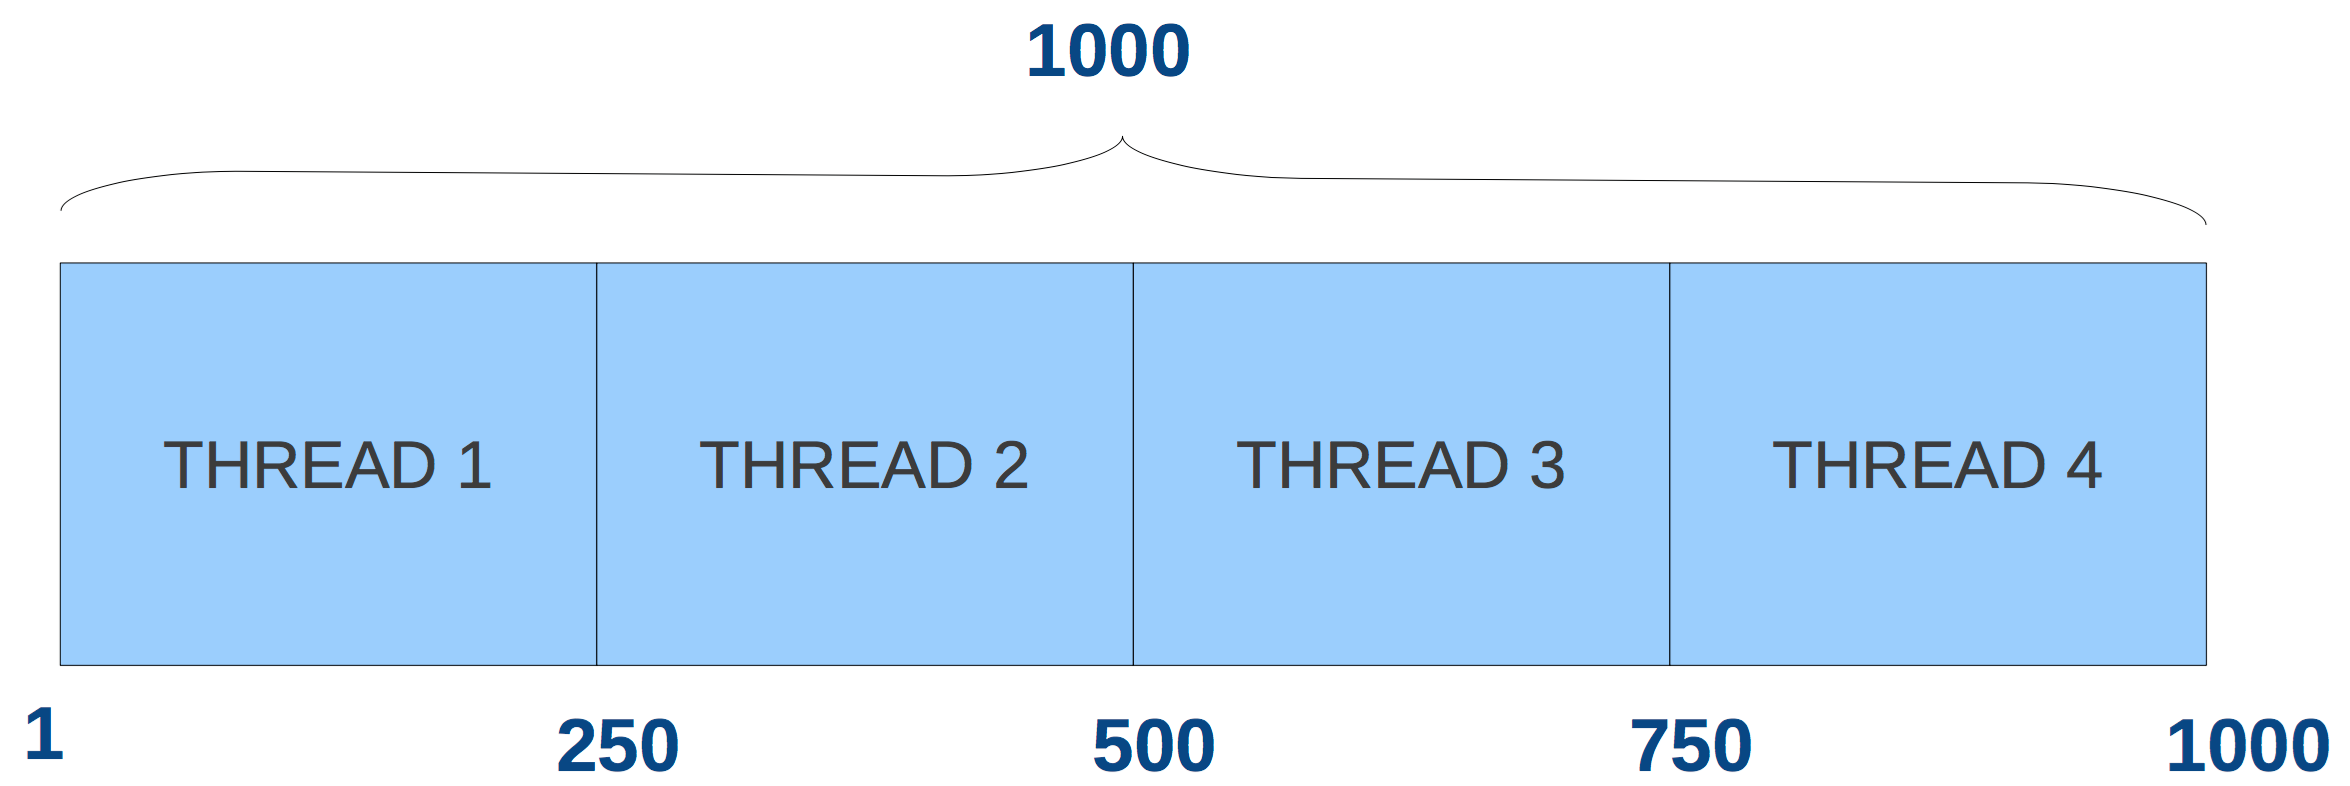
\includegraphics[width=0.5\columnwidth]{PNG/schedule_static.png}
  \caption{ Ilustração do escalonamento estático:}
  \label{fig:schedule_static}
  \end{figure}
}

Ora, esta poderá não ser a melhor forma de escalonamento, muito devido à potencial irregularidade de tempos de conclusão de iteração por cada thread. Em caso de trabalhos regulares esta opção representa o menor overhead do paralelismo. Para casos de um trabalho por iteração por thread com tempos irregulares de conclusão, teremos casos de \textbf{load imbalance}, casos para os quais as opções de escalonamento \textbf{dynamic} e textbf{guided} deverão representar uma melhor solução.\par 

\item \textbf{dynamic} -- O standard OpenMP providência duas formas de escalonamento dinâmico - \textbf{dynamic} e \textbf{guided}, sendo que o último será falado no ponto seguinte. Com escalonamento dinâmico, novas porções de iterações dos ciclos serão atribuídas às threads conforme o trabalho for sendo concluído, sendo essas porções de iterações fixas.\par

\item \textbf{guided} -- com escalonamento guided, novas porções de iterações dos ciclos serão atribuídas às threads conforme o trabalho for sendo concluído, sendo essas porções de iterações dependentes relativas ao número de iterações restantes.\par
\end{itemize}

\subsection{Uma primeira análise ao caso de estudo}
\label{primeiraanalise}
Atente no seguinte excerto de código:
\lstinputlisting[language=C,basicstyle=\scriptsize]{../extra/ex2_v2.cpp} %input de um ficheiro

Que iremos executar para as 3 versões de escalonamento dinâmico especificadas anteriormente, por forma a recolhermos dados estatísticos que nos permitam concluir qual das 3 versões a melhor para o nosso kernel específico.\par
Relativamente às estatísticas teremos interesse em ter conhecimento do momento de criação e término das threads OpenMP, tempos on e off CPU, respectivo número de CPU onde a thread está alocada, assim como as interrupções voluntárias e forçadas e seus tipos.\par 
Assim, o ficheiro \textbf{threaded.d}, disponibilizado no contexto da disciplina, apresenta o seguinte formato:

\lstinputlisting[language=C,basicstyle=\scriptsize]{../extra/threaded_original.d} %input de um ficheiro

Foram ainda realizadas algumas alterações ao mesmo, por forma a facilitar o posterior tratamento da informação, sendo ainda adicionada mais uma probe \textbf{proc:::lwp-exit} por forma a podermos contabilizar o tempo da última operação da thread.\par 
Assim, o ficheiro final utilizado na realização dos testes apresenta o seguinte formato:\par 
\lstinputlisting[language=C,basicstyle=\scriptsize]{../extra/threaded.d} %input de um ficheiro

\subsection{Relação entre o tipo de escalonamento OpenMP, número de Threads OpenMP, e tempo total para a solução, para uma gama de valores aleatórios do ciclo mais interior inalterada ([1:99]).}
\label{tempos_exe3_gama_inalterada}
Com base nos valores impressos pela execução do script dtrace poderemos tratar posteriormente os dados por forma a obtermos uma representação visual, à semelhança do realizado no trabalho prático 2.\par 
Ora, sabendo que o número de Cores físicos de cada CPU é 8, sendo que a máquina em estudo é multiprocessador, totalizando 16 Cores físicos e 32 Cores em HyperThread, devemos realizar os testes que englobem números de threads OpenMP entre 1 e 64. Desta forma, iremos realizar testes para 7 números de threads OpenMP distintos para cada opção de escalonamento, sendo estes 1, 2, 4, 8, 16, 32 e 64 threads.\par 
Inicialmente iremos manter a gama de valores aleatórios do ciclo mais interno do código apresentado na seção \ref{primeiraanalise}. Desta forma garantimos que a distribuição de carga entre threads, qualquer que seja o tipo de escalonamento não irá ser muito distinta. Analisemos portanto essa opção.\par 
Foram realizadas 10 repetições para cada número de Thread OpenMP em teste, e para cada forma de escalonamento. Dessas 10 repetições foi escolhida a que registou um menor tempo total para a solução, produzindo a figura \ref{fig:heatmap_scheduling_openmp}, vulgo \textbf{heatmap}, que associa o número de Threads OpenMP, tipo de escalonamento e Tempo Total para a solução. Denote que cores mais aproximadas do verde escuro representam a melhor solução alcançada:
\begin{figure}[H]
\centering
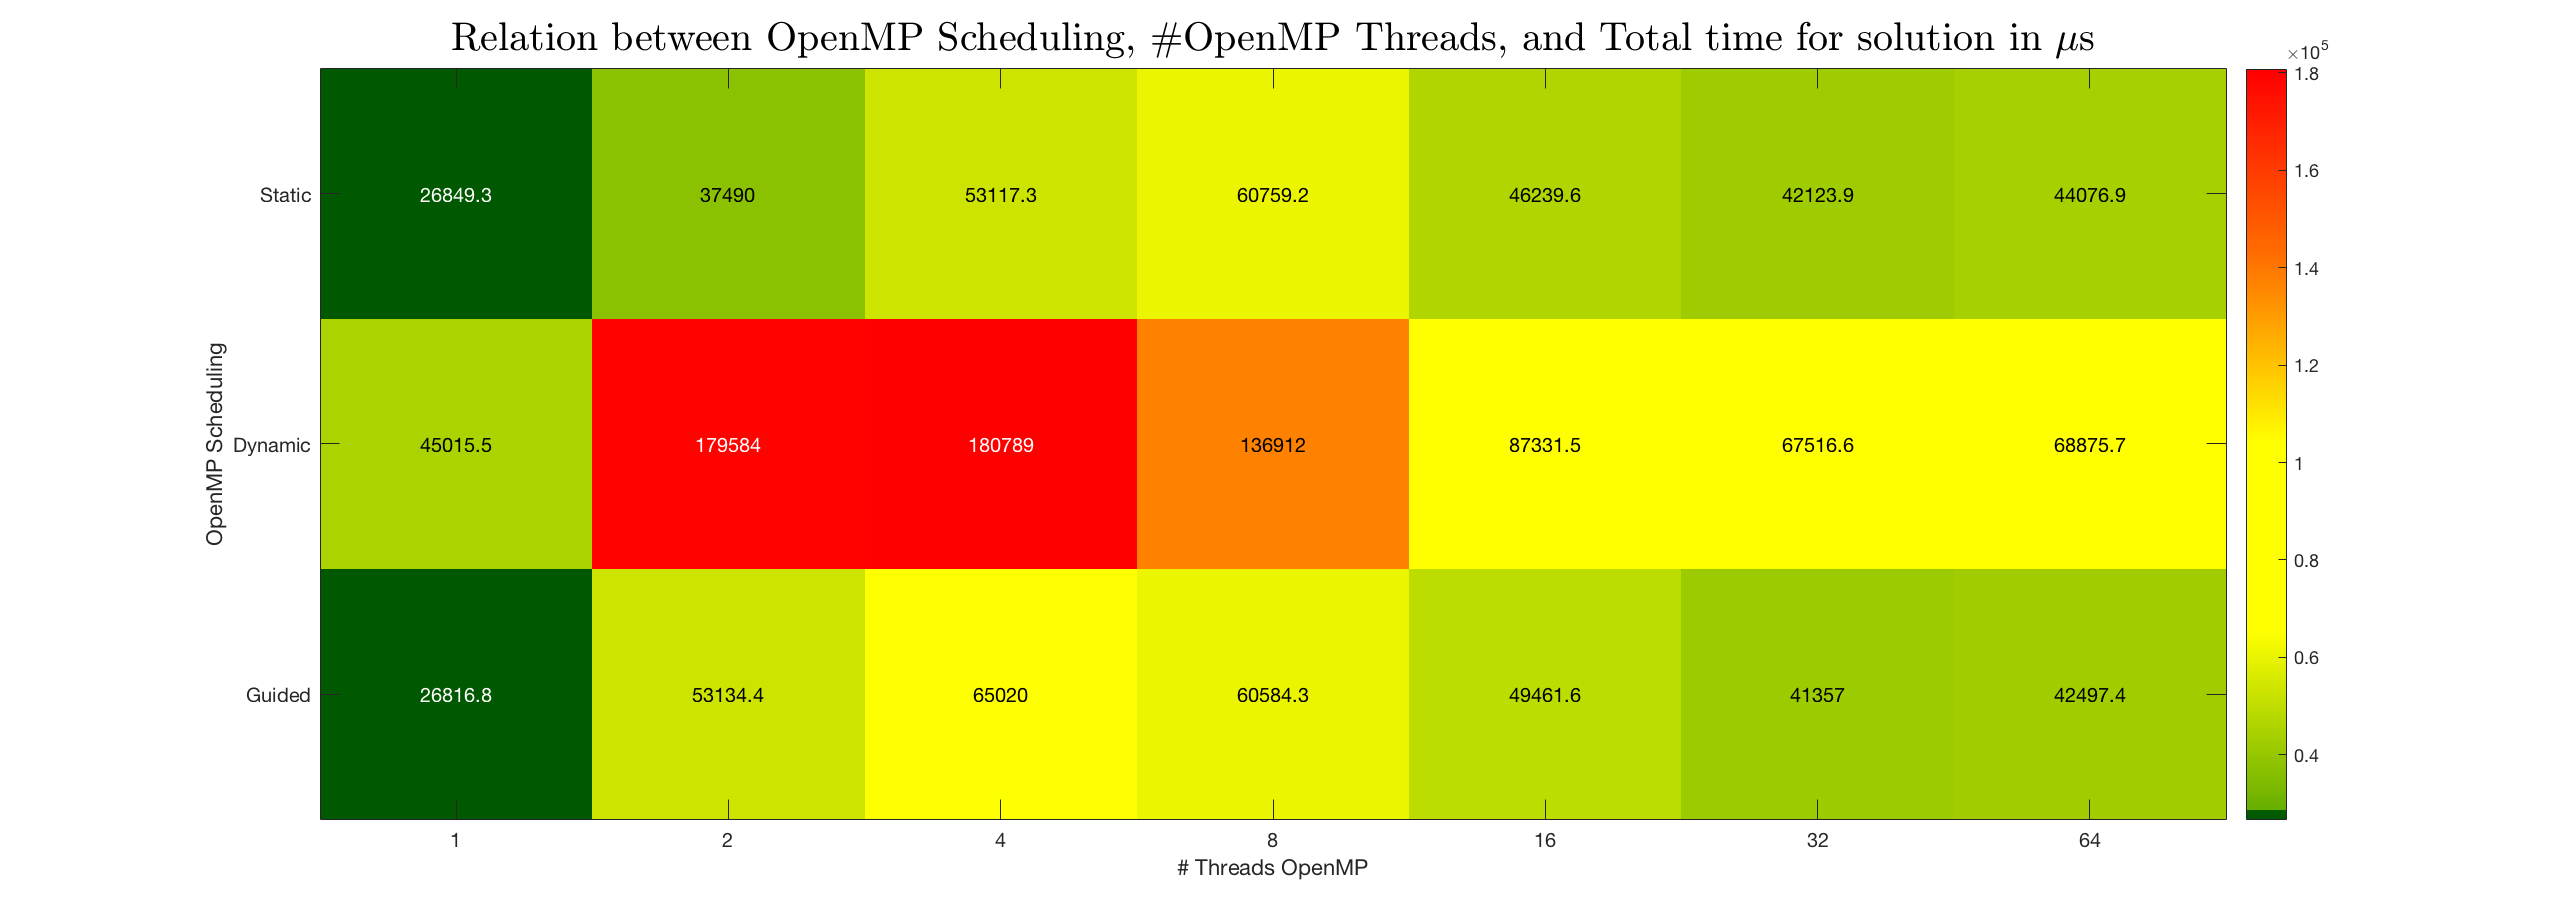
\includegraphics[width=1\columnwidth]{PNG/heatmap_scheduling_openmp.png}
\caption{ Relação entre o tipo de escalonamento OpenMP, número de Threads OpenMP, e tempo total para a solução, para uma gama de valores aleatórios do ciclo mais interior inalterada ([1:99]). }
\label{fig:heatmap_scheduling_openmp}
\end{figure}

\subsubsection{Análise gráfica para o "best-case-scenario" e  "worst-case-scenario" dos tempos totais obtidos no estudo da secção \ref{tempos_exe3_gama_inalterada}}

Voltemos novamente aos valores de tempos totais obtidos e apresentados graficamente na figura \ref{fig:heatmap_scheduling_openmp}. Analisemos portanto os dois outputs produzidos pela ferramenta Dtrace já devidamente ordenados pelo valor da coluna timestamp. Dessa análise resultaram as tabelas \ref{table:static_1_1st_table} e \ref{table:dynamic_4_1st_table}, que apresentaremos de seguida.

\subsubsection{Análise do output da ferramenta Dtrace para o "best-case-scenario" dos tempos totais obtidos no estudo da secção \ref{tempos_exe3_gama_inalterada}}
% !TEX encoding = UTF-8 Unicode

\begin{table}[H]
\caption{Análise do output da ferramenta Dtrace para o "best-case-scenario" dos tempos totais obtidos no estudo da secção \ref{tempos_exe3_gama_inalterada} }
\scriptsize
\label{table:static_1_1st_table}
\centering

\begin{tabular}{ |  L{1.2cm}  |  L{1.2cm}  |  L{0.7cm}  |  L{1cm} |  L{1cm} |  L{1cm} |  L{1cm} |  >{\centering \tiny}m{3cm}  |  L{1.5cm} |  } 
\hline
Timestamp ($\mu$s)        & Delta ($\mu$s)           & TID       & Current CPU  & Current Group & Last CPU  & Last Group & Type                      & Description    \\ \hline
\hline
0              &              & 1         & 7         & 1        &           &          & BEGIN                     &                \\ \hline
895            & 895          & 1         & 24        & 2        & 24        & 2        & CREATE                    &                \\ \hline
906            & 11           & 1         & 24        & 2        & 24        & 2        & RESTART ON SAME CPU       &                \\ \hline
940            & 33           & 1         & 24        & 2        & 24        & 2        & PREEMPTED                 &                \\ \hline
977            & 36           & 1         & 24        & 2        & 24        & 2        & RESTART ON SAME CPU       &                \\ \hline
1423           & 446          & 1         & 24        & 2        & 24        & 2        & PREEMPTED                 &                \\ \hline
2253           & 829          & 1         & 24        & 2        & 24        & 2        & RESTART ON SAME CPU       &                \\ \hline
2267           & 14           & 1         & 24        & 2        & 24        & 2        & PREEMPTED                 &                \\ \hline
2295           & 27           & 1         & 24        & 2        & 24        & 2        & RESTART ON SAME CPU       &                \\ \hline
2535           & 239          & 1         & 24        & 2        & 24        & 2        & PREEMPTED                 &                \\ \hline
2560           & 24           & 1         & 24        & 2        & 24        & 2        & RESTART ON SAME CPU       &                \\ \hline
2569           & 9            & 1         & 24        & 2        & 24        & 2        & PREEMPTED                 &                \\ \hline
2604           & 35           & 1         & 24        & 2        & 24        & 2        & RESTART ON SAME CPU       &                \\ \hline
32506          & 29901        & 1         & 24        & 2        & 24        & 2        & SLEEPING ON               & cond var       \\ \hline
32524          & 18           & 1         & 24        & 2        & 24        & 2        & PREEMPTED                 &                \\ \hline
34663          & 2138         & 1         & 24        & 2        & 24        & 2        & RESTART ON SAME CPU       &                \\ \hline
34718          & 55           & 1         & 24        & 2        & 24        & 2        & SLEEPING ON               & cond var       \\ \hline
34724          & 5            & 1         & 24        & 2        & 24        & 2        & PREEMPTED                 &                \\ \hline
34888          & 164          & 1         & 24        & 2        & 24        & 2        & RESTART ON SAME CPU       &                \\ \hline
34931          & 42           & 1         & 24        & 2        & 24        & 2        & SLEEPING ON               & shuttle        \\ \hline
34936          & 4            & 1         & 24        & 2        & 24        & 2        & PREEMPTED                 &                \\ \hline
34991          & 54           & 1         & 24        & 2        & 24        & 2        & RESTART ON SAME CPU       &                \\ \hline
35001          & 10           & 1         & 24        & 2        & 24        & 2        & SLEEPING ON               & shuttle        \\ \hline
35005          & 4            & 1         & 24        & 2        & 24        & 2        & PREEMPTED                 &                \\ \hline
35031          & 25           & 1         & 24        & 2        & 24        & 2        & RESTART ON SAME CPU       &                \\ \hline
35174          & 143          & 1         & 24        & 2        & 24        & 2        & EXIT                      &                \\ \hline
35329          &              & 1         & 7         & 1        &           &          & END                       &                \\ \hline
\end{tabular}
\end{table}


\subsubsection{Análise do output da ferramenta Dtrace para o "worst-case-scenario" dos tempos totais obtidos no estudo da secção \ref{tempos_exe3_gama_inalterada}}
% !TEX encoding = UTF-8 Unicode

\begin{table}[H]
\caption{Análise do output da ferramenta Dtrace para o "worst-case-scenario" dos tempos totais obtidos no estudo da secção \ref{tempos_exe3_gama_inalterada} }
\scriptsize
\label{table:dynamic_4_1st_table}
\centering

\begin{tabular}{ |  L{1.2cm}  |  L{1.2cm}  |  L{0.7cm}  |  L{1cm} |  L{1cm} |  L{1cm} |  L{1cm} |  >{\centering \tiny}m{3cm}  |  L{1.5cm} |  } 
\hline
Timestamp ($\mu$s)        & Delta ($\mu$s)           & TID       & Current CPU  & Current Group & Last CPU  & Last Group & Type                      & Description    \\ \hline
\hline
0                     &                      & 1         & 2         & 1        &           &          & BEGIN                     &                \\ \hline
803                   & 803                  & 1         & 14        & 2        & 14        & 2        & CREATE                    &                \\ \hline
831                   & 28                   & 1         & 14        & 2        & 14        & 2        & RESTART ON SAME CPU       &                \\ \hline
867                   & 35                   & 1         & 14        & 2        & 14        & 2        & PREEMPTED                 &                \\ \hline
936                   & 68                   & 1         & 14        & 2        & 14        & 2        & RESTART ON SAME CPU       &                \\ \hline
1411                  & 475                  & 1         & 14        & 2        & 14        & 2        & PREEMPTED                 &                \\ \hline
2072                  & 661                  & 1         & 14        & 2        & 14        & 2        & RESTART ON SAME CPU       &                \\ \hline
2132                  & 59                   & 1         & 14        & 2        & 14        & 2        & PREEMPTED                 &                \\ \hline
2158                  & 25                   & 1         & 14        & 2        & 14        & 2        & RESTART ON SAME CPU       &                \\ \hline
2398                  & 239                  & 1         & 14        & 2        & 14        & 2        & PREEMPTED                 &                \\ \hline
2444                  & 46                   & 1         & 14        & 2        & 14        & 2        & RESTART ON SAME CPU       &                \\ \hline
2470                  & 26                   & 1         & 14        & 2        & 14        & 2        & PREEMPTED                 &                \\ \hline
2513                  & 43                   & 1         & 14        & 2        & 14        & 2        & RESTART ON SAME CPU       &                \\ \hline
6192                  & 6192                 & 3         & 13        & 2        & 13        & 2        & CREATE                    &                \\ \hline
6197                  & 6197                 & 2         & 7         & 1        & 7         & 1        & CREATE                    &                \\ \hline
6198                  & 6                    & 3         & 13        & 2        & 13        & 2        & RESTART ON SAME CPU       &                \\ \hline
6208                  & 3694                 & 1         & 14        & 2        & 14        & 2        & SLEEPING ON               & cond var       \\ \hline
6212                  & 15                   & 2         & 7         & 1        & 7         & 1        & RESTART ON SAME CPU       &                \\ \hline
6216                  & 17                   & 3         & 13        & 2        & 13        & 2        & SLEEPING ON               & cond var       \\ \hline
6220                  & 12                   & 1         & 14        & 2        & 14        & 2        & PREEMPTED                 &                \\ \hline
6223                  & 7                    & 3         & 13        & 2        & 13        & 2        & PREEMPTED                 &                \\ \hline
6251                  & 6251                 & 4         & 21        & 1        & 21        & 1        & CREATE                    &                \\ \hline
6257                  & 5                    & 4         & 21        & 1        & 21        & 1        & RESTART ON SAME CPU       &                \\ \hline
6262                  & 49                   & 2         & 7         & 1        & 7         & 1        & SLEEPING ON               & cond var       \\ \hline
6272                  & 9                    & 2         & 7         & 1        & 7         & 1        & PREEMPTED                 &                \\ \hline
6287                  & 29                   & 4         & 21        & 1        & 21        & 1        & SLEEPING ON               & cond var       \\ \hline
6291                  & 70                   & 1         & 14        & 2        & 14        & 2        & RESTART ON SAME CPU       &                \\ \hline
6295                  & 8                    & 4         & 21        & 1        & 21        & 1        & PREEMPTED                 &                \\ \hline
6305                  & 82                   & 3         & 13        & 2        & 13        & 2        & RESTART ON SAME CPU       &                \\ \hline
6345                  & 72                   & 2         & 7         & 1        & 7         & 1        & RESTART ON SAME CPU       &                \\ \hline
6393                  & 97                   & 4         & 21        & 1        & 21        & 1        & RESTART ON SAME CPU       &                \\ \hline
186405                & 180012               & 4         & 21        & 1        & 21        & 1        & SLEEPING ON               & cond var       \\ \hline
186410                & 180065               & 2         & 7         & 1        & 7         & 1        & SLEEPING ON               & cond var       \\ \hline
186413                & 8                    & 4         & 21        & 1        & 21        & 1        & PREEMPTED                 &                \\ \hline
186414                & 180108               & 3         & 13        & 2        & 13        & 2        & SLEEPING ON               & cond var       \\ \hline
186419                & 180127               & 1         & 14        & 2        & 14        & 2        & SLEEPING ON               & cond var       \\ \hline
186419                & 8                    & 2         & 7         & 1        & 7         & 1        & PREEMPTED                 &                \\ \hline
186421                & 7                    & 3         & 13        & 2        & 13        & 2        & PREEMPTED                 &                \\ \hline
186424                & 5                    & 1         & 14        & 2        & 14        & 2        & PREEMPTED                 &                \\ \hline
186425                & 11                   & 4         & 21        & 1        & 21        & 1        & RESTART ON SAME CPU       &                \\ \hline
186438                & 19                   & 2         & 7         & 1        & 7         & 1        & RESTART ON SAME CPU       &                \\ \hline
186439                & 14                   & 4         & 21        & 1        & 21        & 1        & SLEEPING ON               & cond var       \\ \hline
186446                & 6                    & 4         & 21        & 1        & 21        & 1        & PREEMPTED                 &                \\ \hline
186448                & 9                    & 2         & 7         & 1        & 7         & 1        & SLEEPING ON               & cond var       \\ \hline
186461                & 12                   & 2         & 7         & 1        & 7         & 1        & PREEMPTED                 &                \\ \hline
186469                & 47                   & 3         & 13        & 2        & 13        & 2        & RESTART ON SAME CPU       &                \\ \hline
186504                & 35                   & 3         & 13        & 2        & 13        & 2        & SLEEPING ON               & cond var       \\ \hline
186506                & 81                   & 1         & 14        & 2        & 14        & 2        & RESTART ON SAME CPU       &                \\ \hline
186528                & 23                   & 3         & 13        & 2        & 13        & 2        & PREEMPTED                 &                \\ \hline
186659                & 152                  & 1         & 14        & 2        & 14        & 2        & SLEEPING ON               & cond var       \\ \hline
186666                & 7                    & 1         & 14        & 2        & 14        & 2        & PREEMPTED                 &                \\ \hline
188662                & 1995                 & 1         & 14        & 2        & 14        & 2        & RESTART ON SAME CPU       &                \\ \hline
188717                & 54                   & 1         & 14        & 2        & 14        & 2        & SLEEPING ON               & cond var       \\ \hline
188723                & 5                    & 1         & 14        & 2        & 14        & 2        & PREEMPTED                 &                \\ \hline
188899                & 176                  & 1         & 14        & 2        & 14        & 2        & RESTART ON SAME CPU       &                \\ \hline
188934                & 34                   & 1         & 14        & 2        & 14        & 2        & SLEEPING ON               & shuttle        \\ \hline
188958                & 23                   & 1         & 14        & 2        & 14        & 2        & PREEMPTED                 &                \\ \hline
189022                & 64                   & 1         & 14        & 2        & 14        & 2        & RESTART ON SAME CPU       &                \\ \hline
189033                & 10                   & 1         & 14        & 2        & 14        & 2        & SLEEPING ON               & shuttle        \\ \hline
189037                & 4                    & 1         & 14        & 2        & 14        & 2        & PREEMPTED                 &                \\ \hline
189057                & 19                   & 1         & 14        & 2        & 14        & 2        & RESTART ON SAME CPU       &                \\ \hline
189228                & 171                  & 1         & 14        & 2        & 14        & 2        & SLEEPING ON               & cond var       \\ \hline
189228                & 2700                 & 3         & 13        & 2        & 13        & 2        & RESTART ON SAME CPU       &                \\ \hline
189229                & 2767                 & 2         & 7         & 1        & 7         & 1        & RESTART ON SAME CPU       &                \\ \hline
189231                & 2784                 & 4         & 21        & 1        & 21        & 1        & RESTART ON SAME CPU       &                \\ \hline
189235                & 7                    & 1         & 14        & 2        & 14        & 2        & PREEMPTED                 &                \\ \hline
189238                & 10                   & 3         & 13        & 2        & 13        & 2        & EXIT                      &                \\ \hline
189264                & 34                   & 2         & 7         & 1        & 7         & 1        & EXIT                      &                \\ \hline
189265                & 30                   & 1         & 14        & 2        & 14        & 2        & RESTART ON SAME CPU       &                \\ \hline
189274                & 8                    & 1         & 14        & 2        & 14        & 2        & SLEEPING ON               & cond var       \\ \hline
189280                & 49                   & 4         & 21        & 1        & 21        & 1        & EXIT                      &                \\ \hline
189280                & 5                    & 1         & 14        & 2        & 14        & 2        & PREEMPTED                 &                \\ \hline
189293                & 12                   & 1         & 14        & 2        & 14        & 2        & RESTART ON SAME CPU       &                \\ \hline
189298                & 4                    & 1         & 14        & 2        & 14        & 2        & EXIT                      &                \\ \hline
189485                &                      & 1         & 2         & 1        &           &          & END                       &                \\ \hline
\end{tabular}
\end{table}




\subsubsection{Análise gráfica para o "best-case-scenario" dos tempos totais obtidos no estudo da secção \ref{tempos_exe3_gama_inalterada}}

Ora, retomando o exemplo do trabalho prático 2, e da análise gráfica da criação e término de threads, será interessante compreender a influência de cada uma das \textbf{probes} adicionadas ao profiling no comportamento da melhor e pior versões da aplicação. \par
Desta forma, foram produzidas as figuras \ref{fig:worst_dynamic_4_threads} a \ref{fig:worst_dynamic_4_threads_again}, ilustrando o descrito anteriormente, permitindo ainda a comparação com a mesma escala de tempos as duas versões da aplicação.\par 


\begin{figure}[H]
\centering
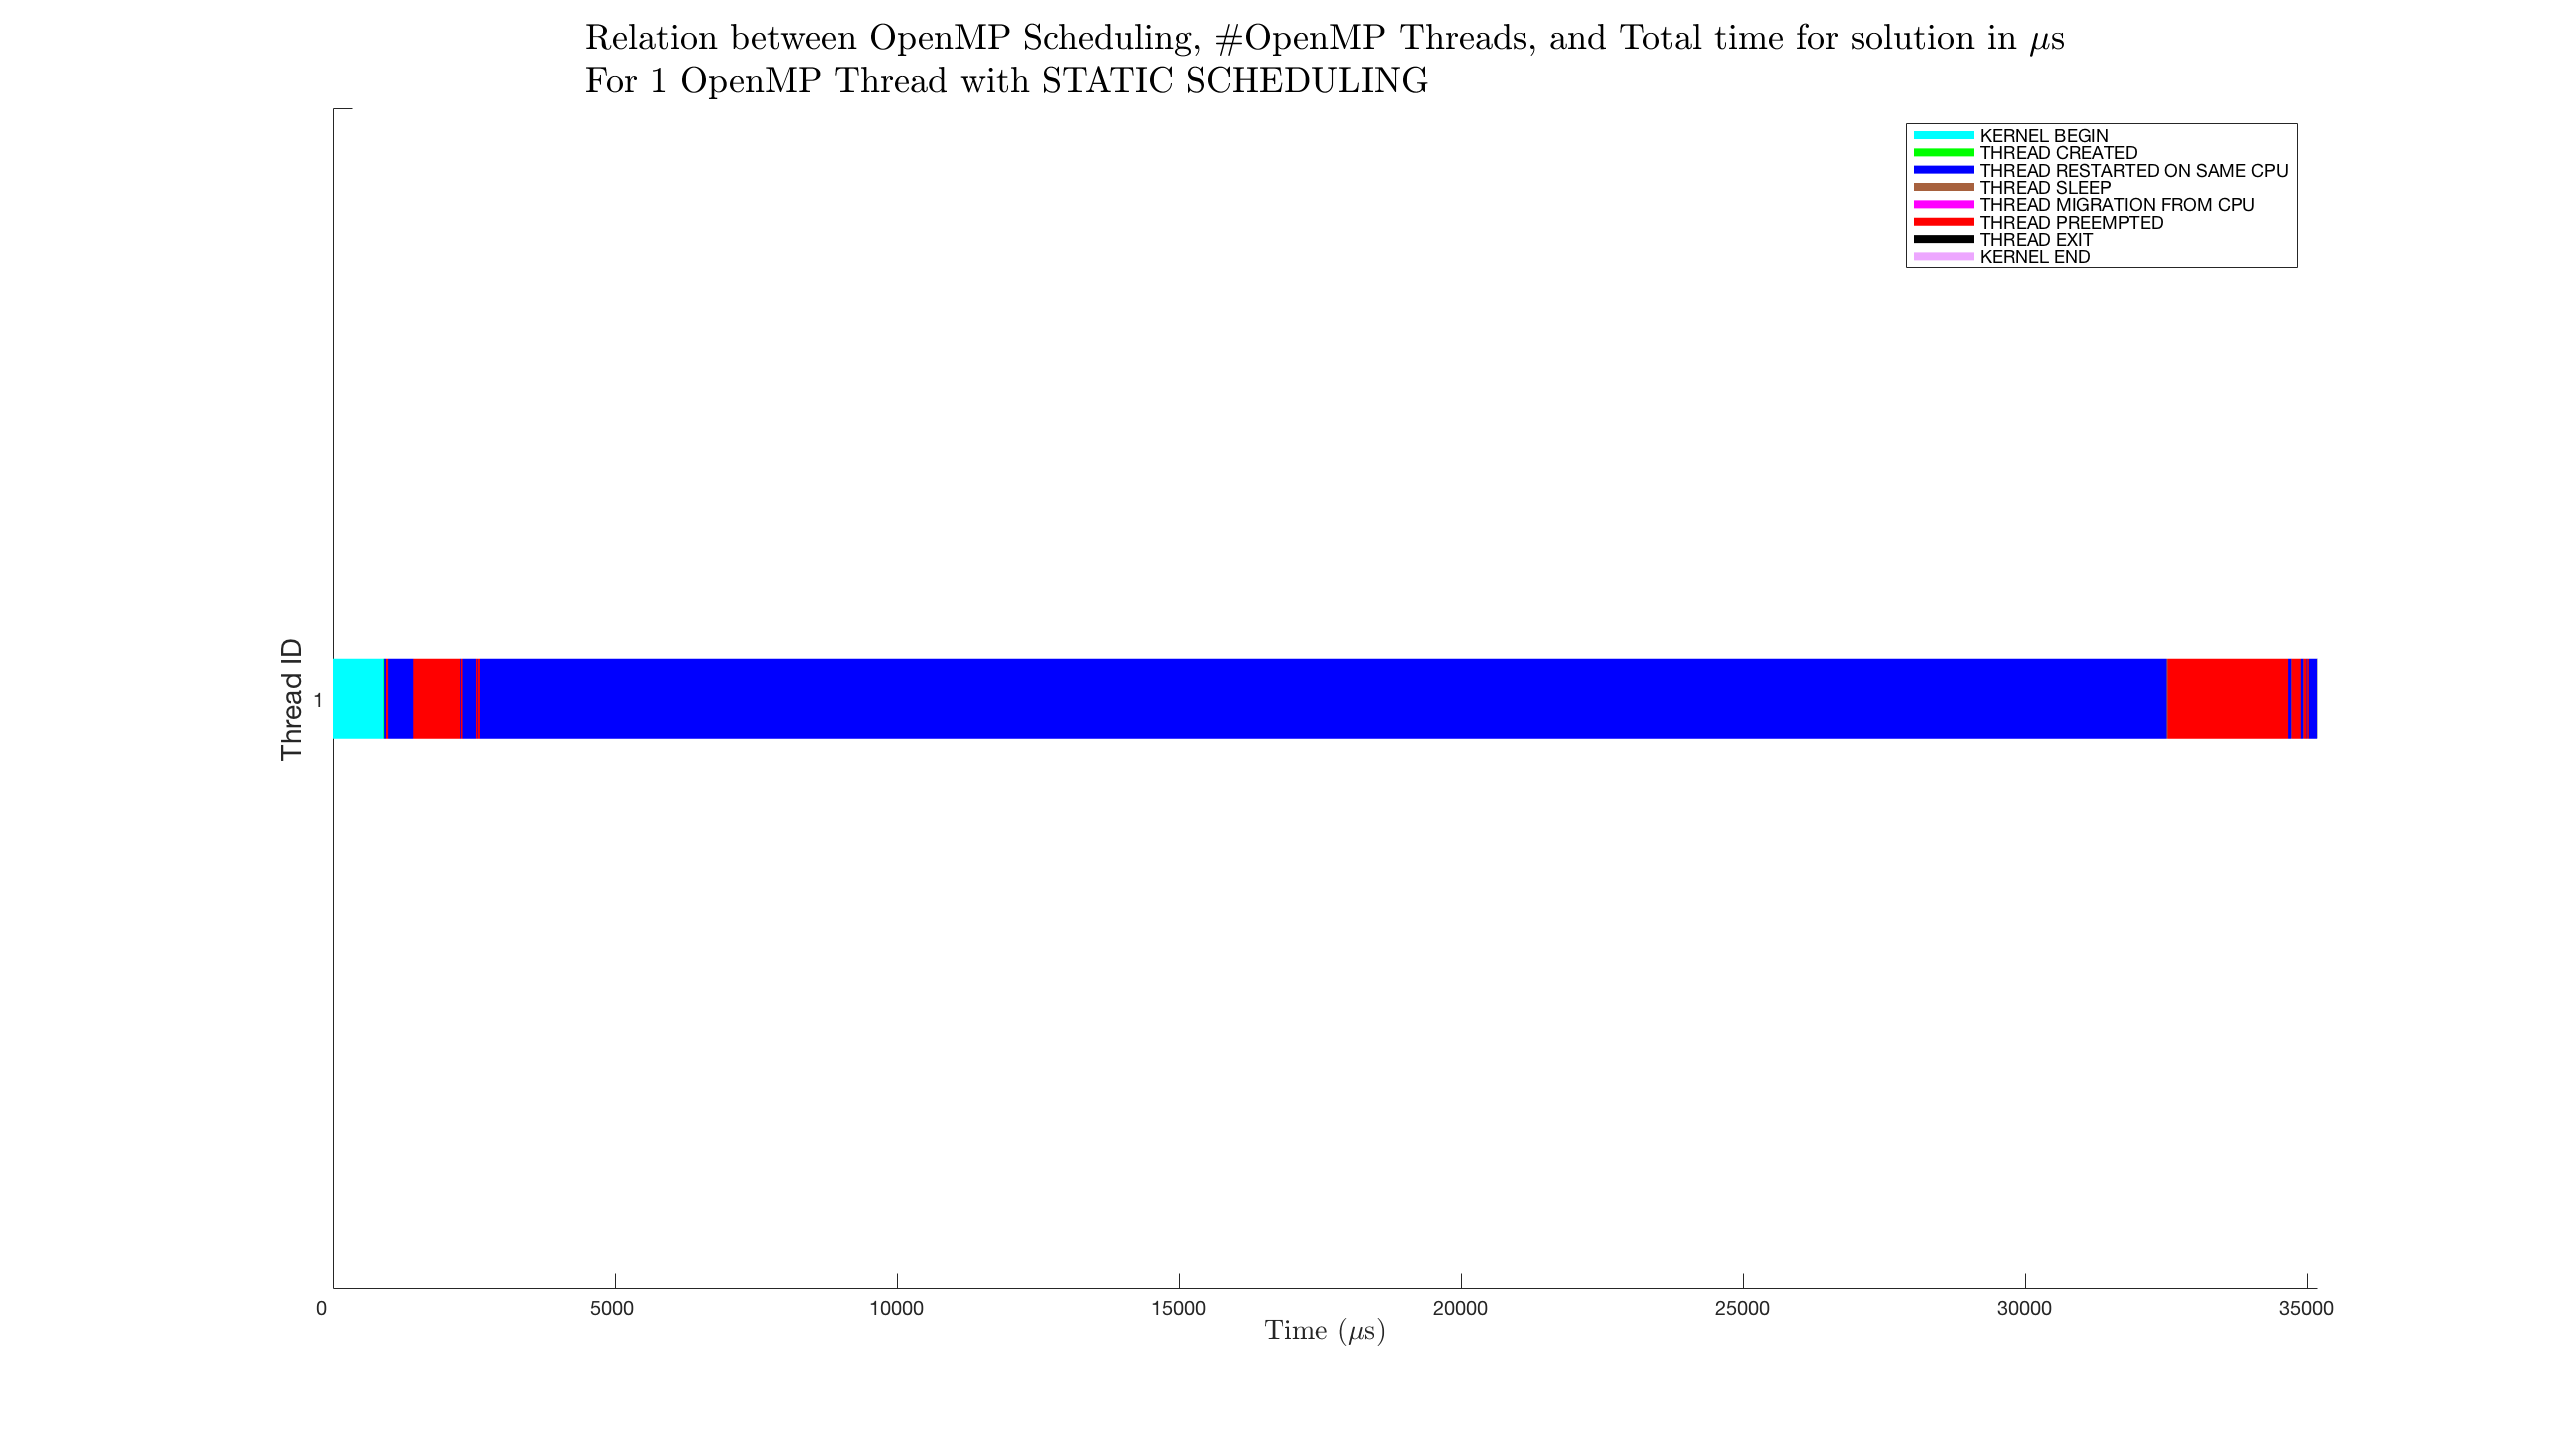
\includegraphics[width=0.9\columnwidth]{PNG/best_static_1_thread.png}
\caption{ Análise gráfica para o "best-case-scenario" dos tempos totais obtidos no estudo da secção \ref{tempos_exe3_gama_inalterada}, para uma gama de valores aleatórios do ciclo mais interior inalterada ([1:99]). }
\label{fig:best_static_1_thread}
\end{figure}


\subsubsection{Análise gráfica para o "worst-case-scenario" dos tempos totais obtidos no estudo da secção \ref{tempos_exe3_gama_inalterada}}



\begin{figure}[H]
\centering
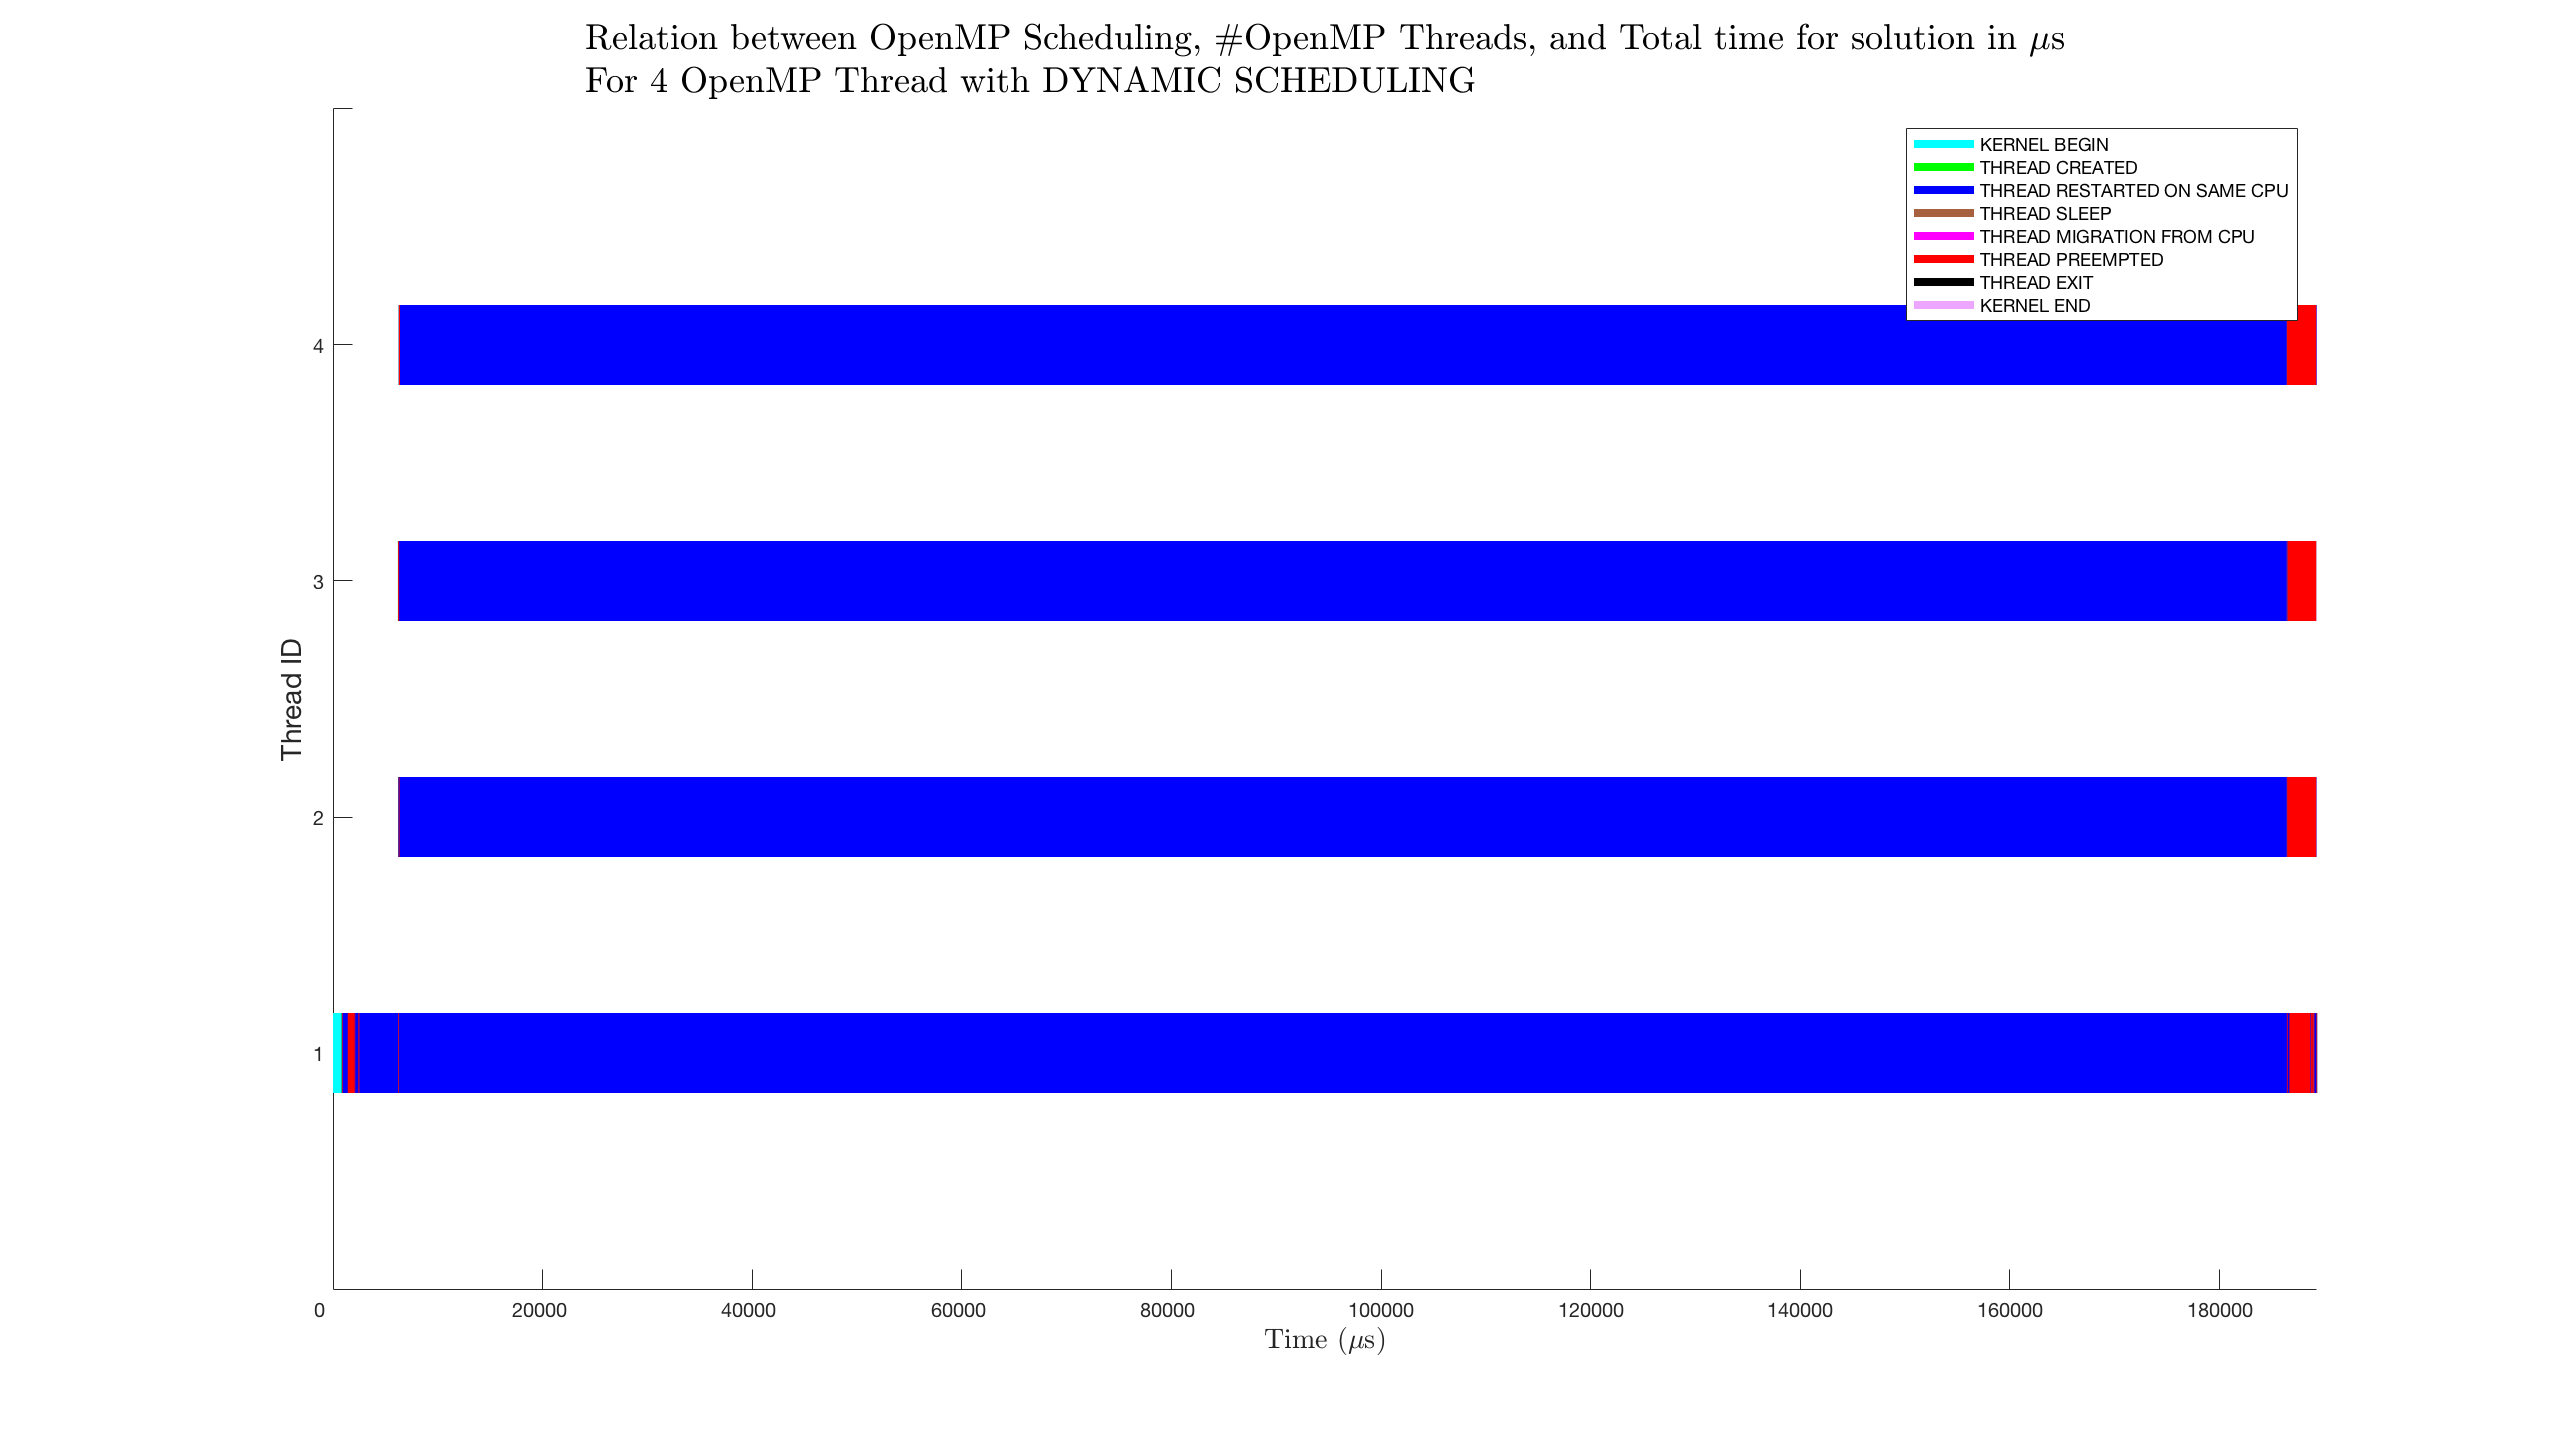
\includegraphics[width=0.9\columnwidth]{PNG/worst_dynamic_4_threads.png}
\caption{ Análise gráfica para o "worst-case-scenario" dos tempos totais obtidos no estudo da secção \ref{tempos_exe3_gama_inalterada}, para uma gama de valores aleatórios do ciclo mais interior inalterada ([1:99]). }
\label{fig:worst_dynamic_4_threads}
\end{figure}

\newpage


\begin{figure}[H]
\centering
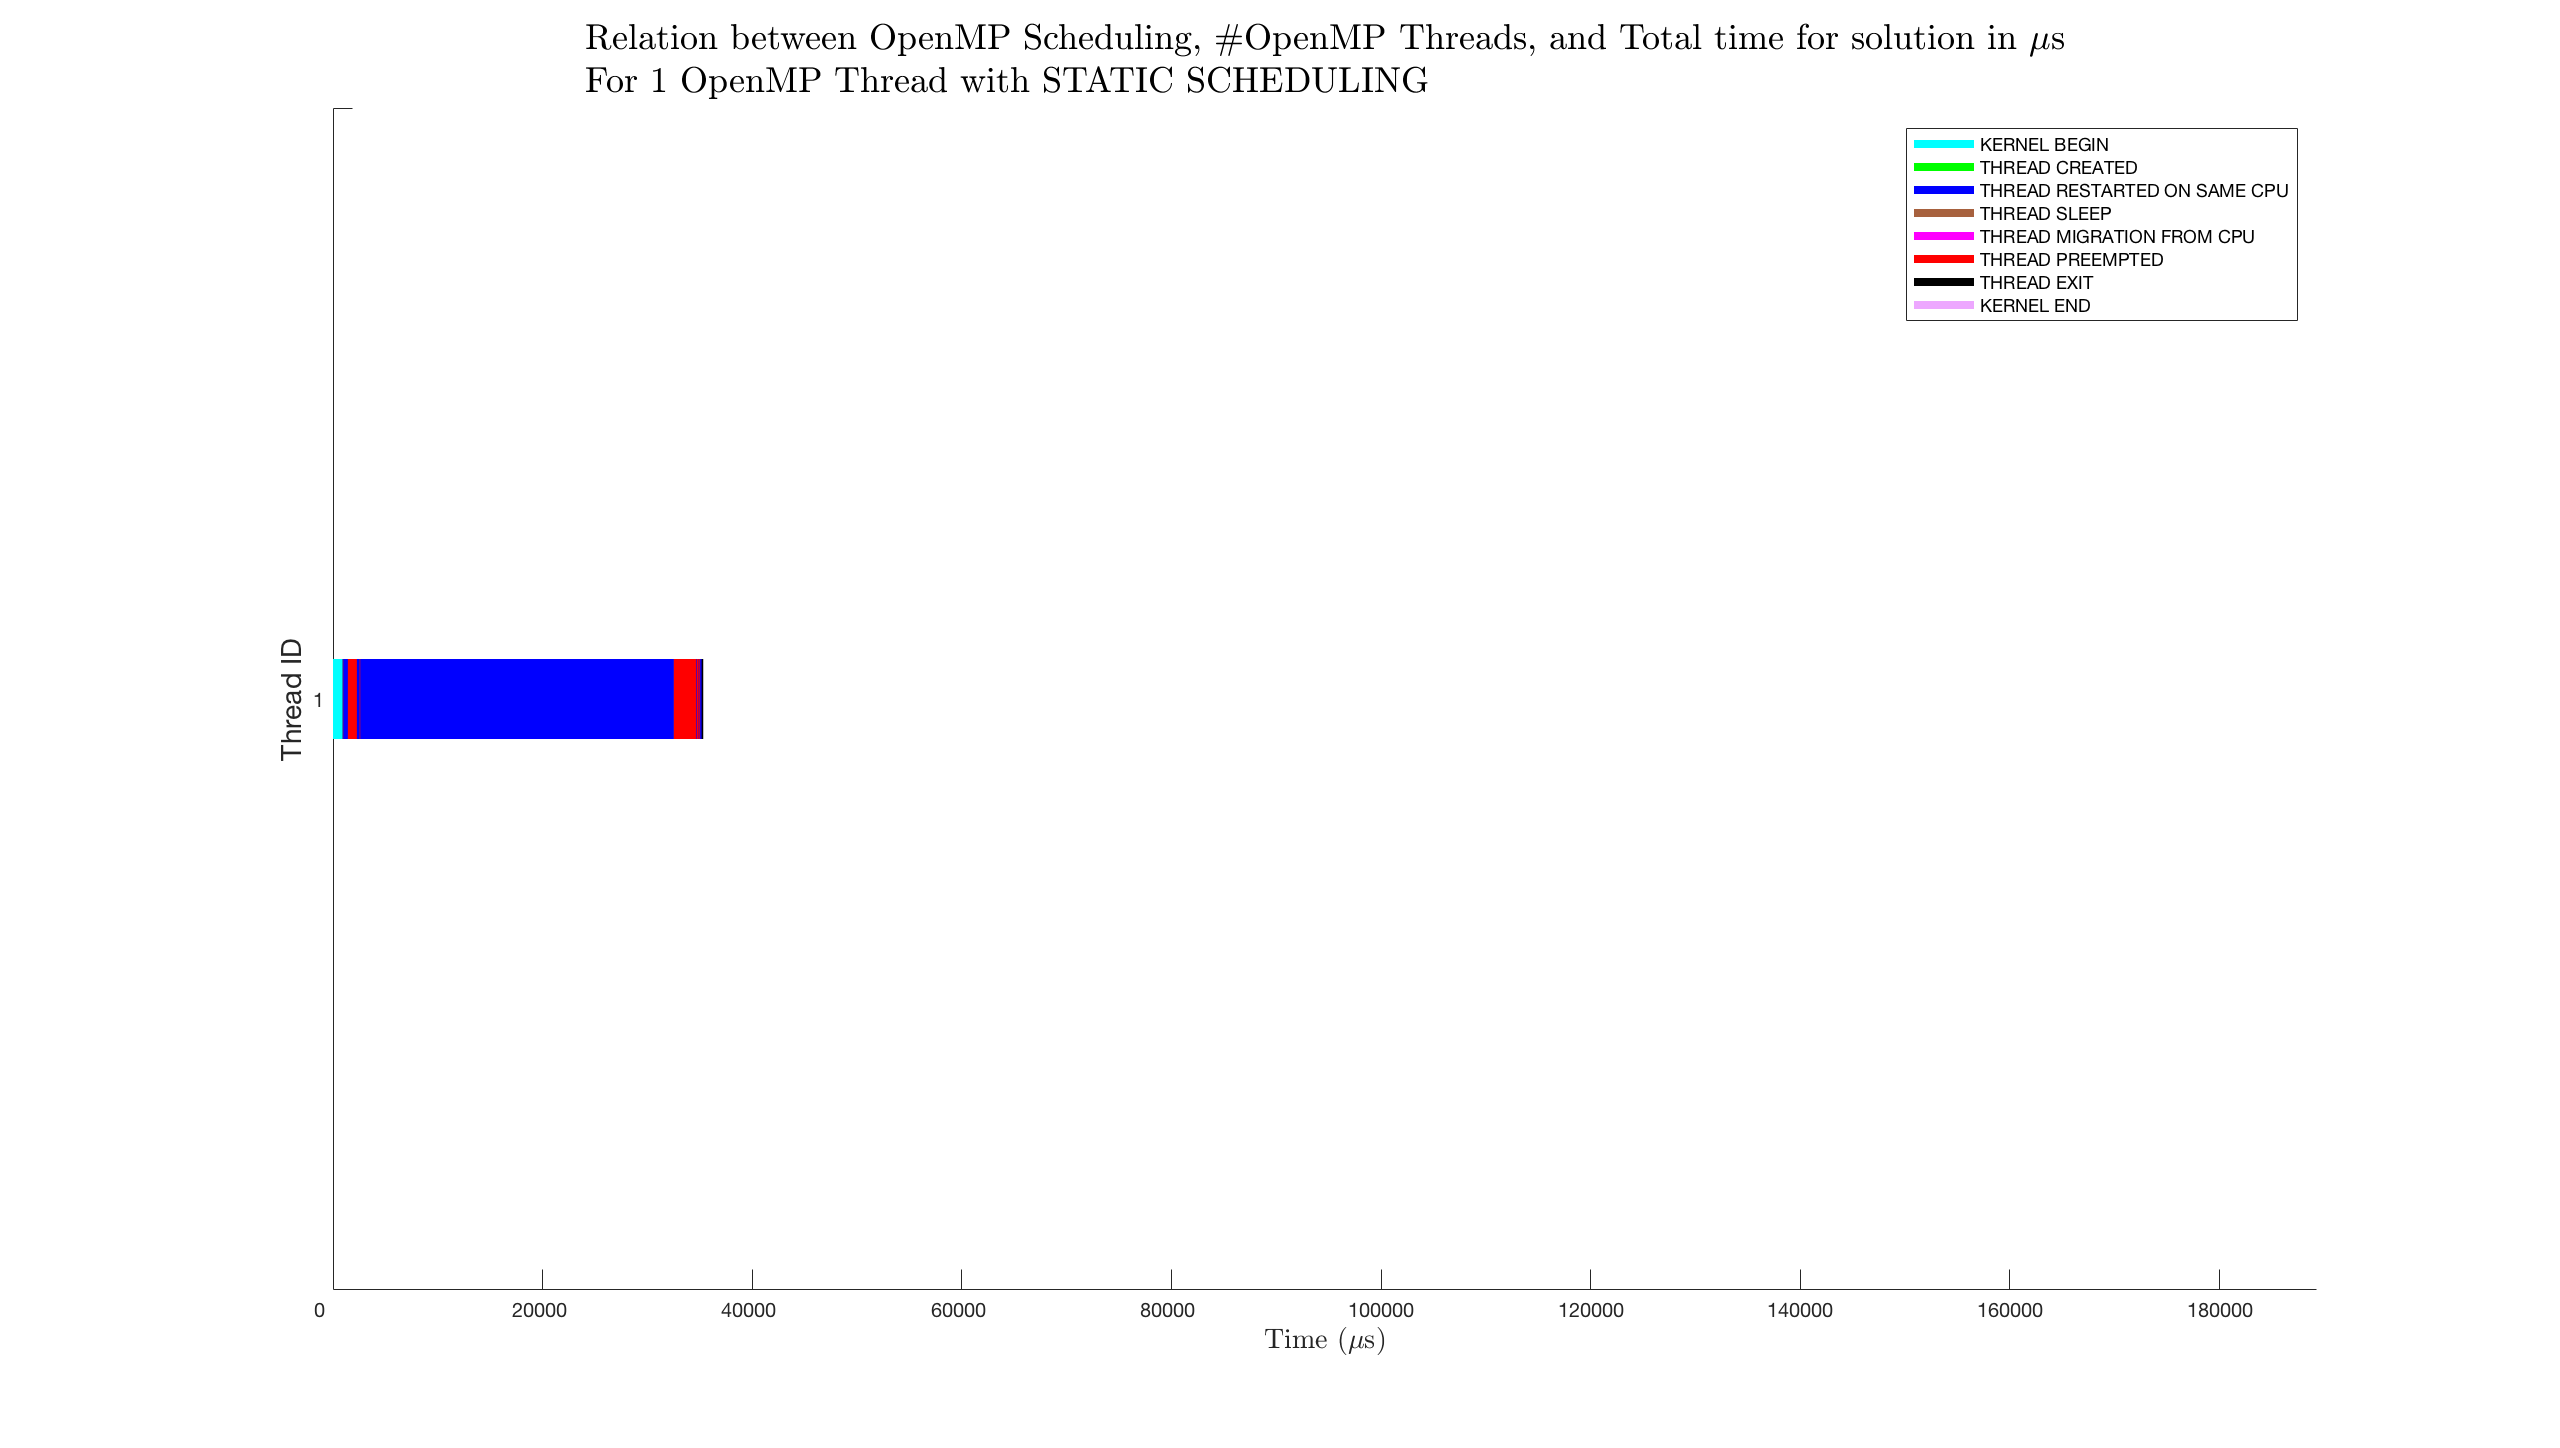
\includegraphics[width=1\columnwidth]{PNG/best_static_1_thread_scaled.png}
\caption{ Análise gráfica para o "best-case-scenario" dos tempos totais obtidos no estudo da secção \ref{tempos_exe3_gama_inalterada}, para uma gama de valores aleatórios do ciclo mais interior inalterada ([1:99]), com a mesma escala de tempos presente para o "worst-case-scenario". }
\label{fig:best_static_1_thread_scaled}
\end{figure}

\begin{figure}[H]
\centering
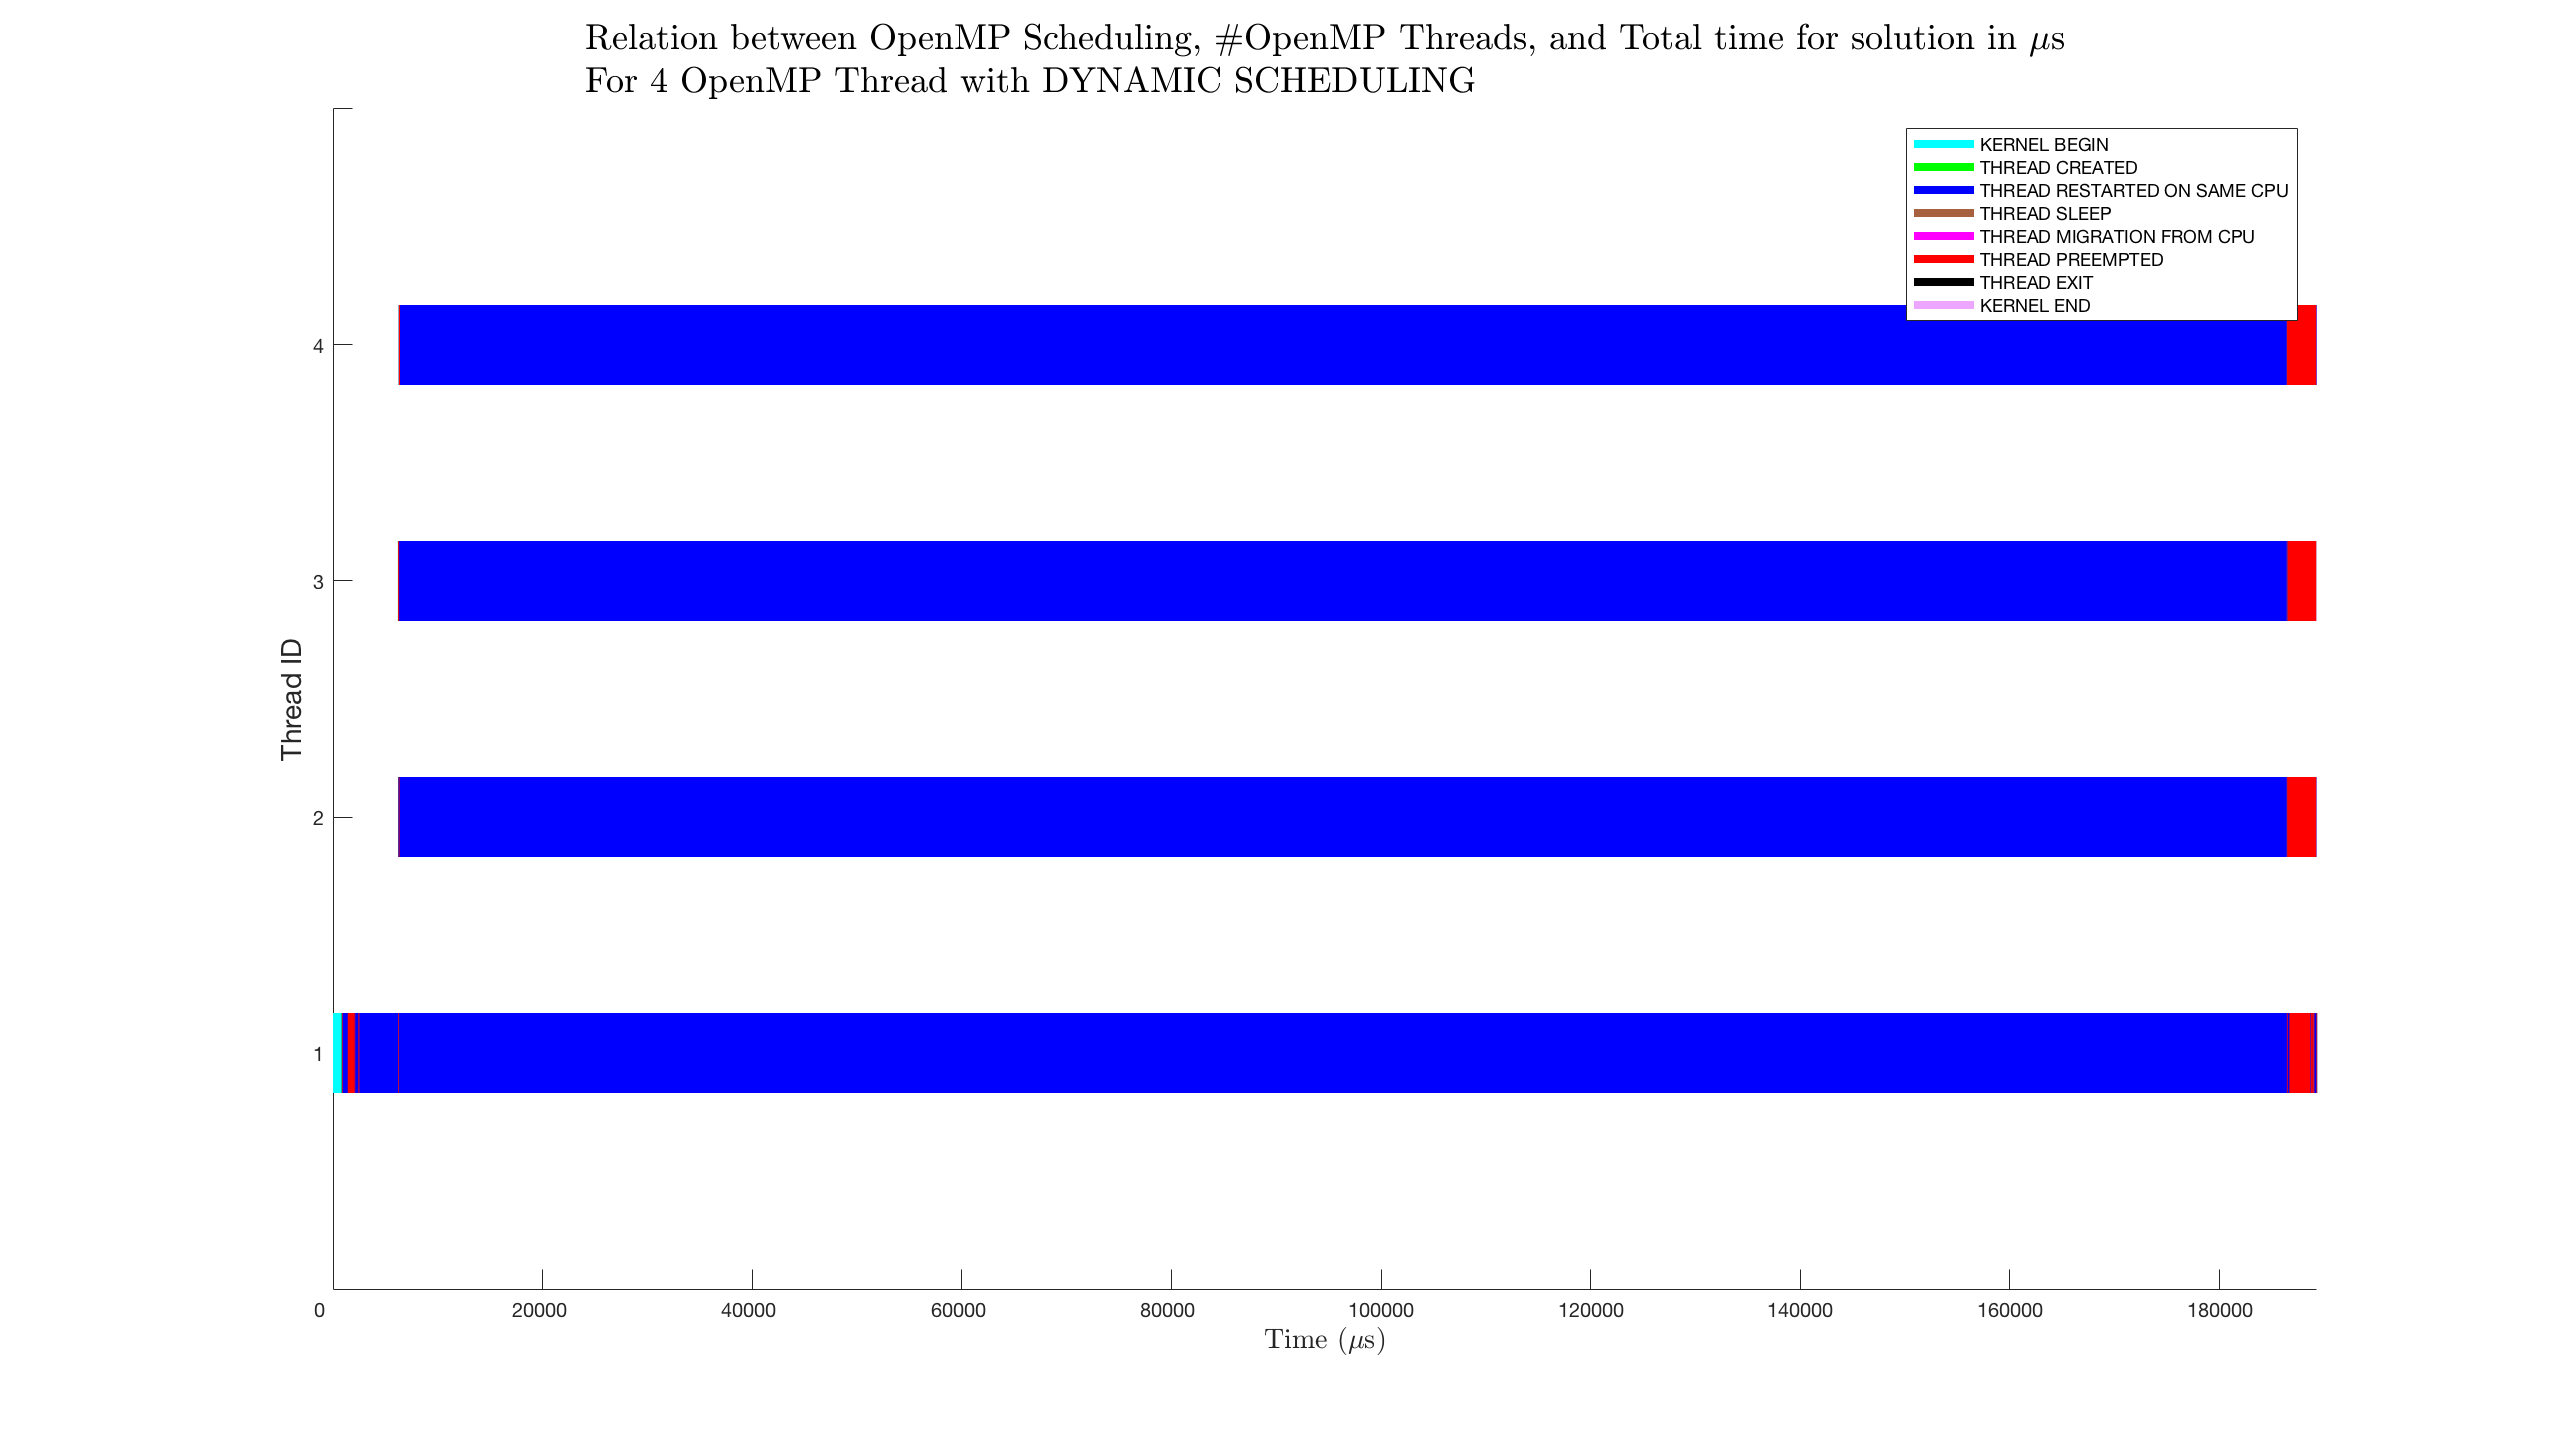
\includegraphics[width=1\columnwidth]{PNG/worst_dynamic_4_threads.png}
\caption{ Análise gráfica para o "worst-case-scenario" dos tempos totais obtidos no estudo da secção \ref{tempos_exe3_gama_inalterada}, para uma gama de valores aleatórios do ciclo mais interior inalterada ([1:99]). }
\label{fig:worst_dynamic_4_threads_again}
\end{figure}

Tendo em conta a dimensão da LLCache da máquina de teste, e a respectiva dimensão do dataset em estudo, conseguimos garantir que durante a computação, não existem bootlenecks "memory related". Ora, pela análise das imagens anteriores compreendemos que o grande diferenciador entre ambas as versões é respectivamente o overhead adicional da zona paralela. Se por uma lado, para escalonamento estático temos um menor overhead, para o caso do escalonamento dinâmico, esse mesmo overhead é completamente limitante em termos de performance. \par 
Ora, esta análise depreende que os valores aleatórios do ciclo interno se encontram num intervalo de valores muito restrito, e é por essa mesma razão que o escalonamento estático não sofre de load imbalance quando comparado com outros tipos de escalonamento. \par Testemos agora a situação onde o intervalo de valores poderá estar compreendido entre [1 e  262144 ].

\begin{figure}[H]
\centering
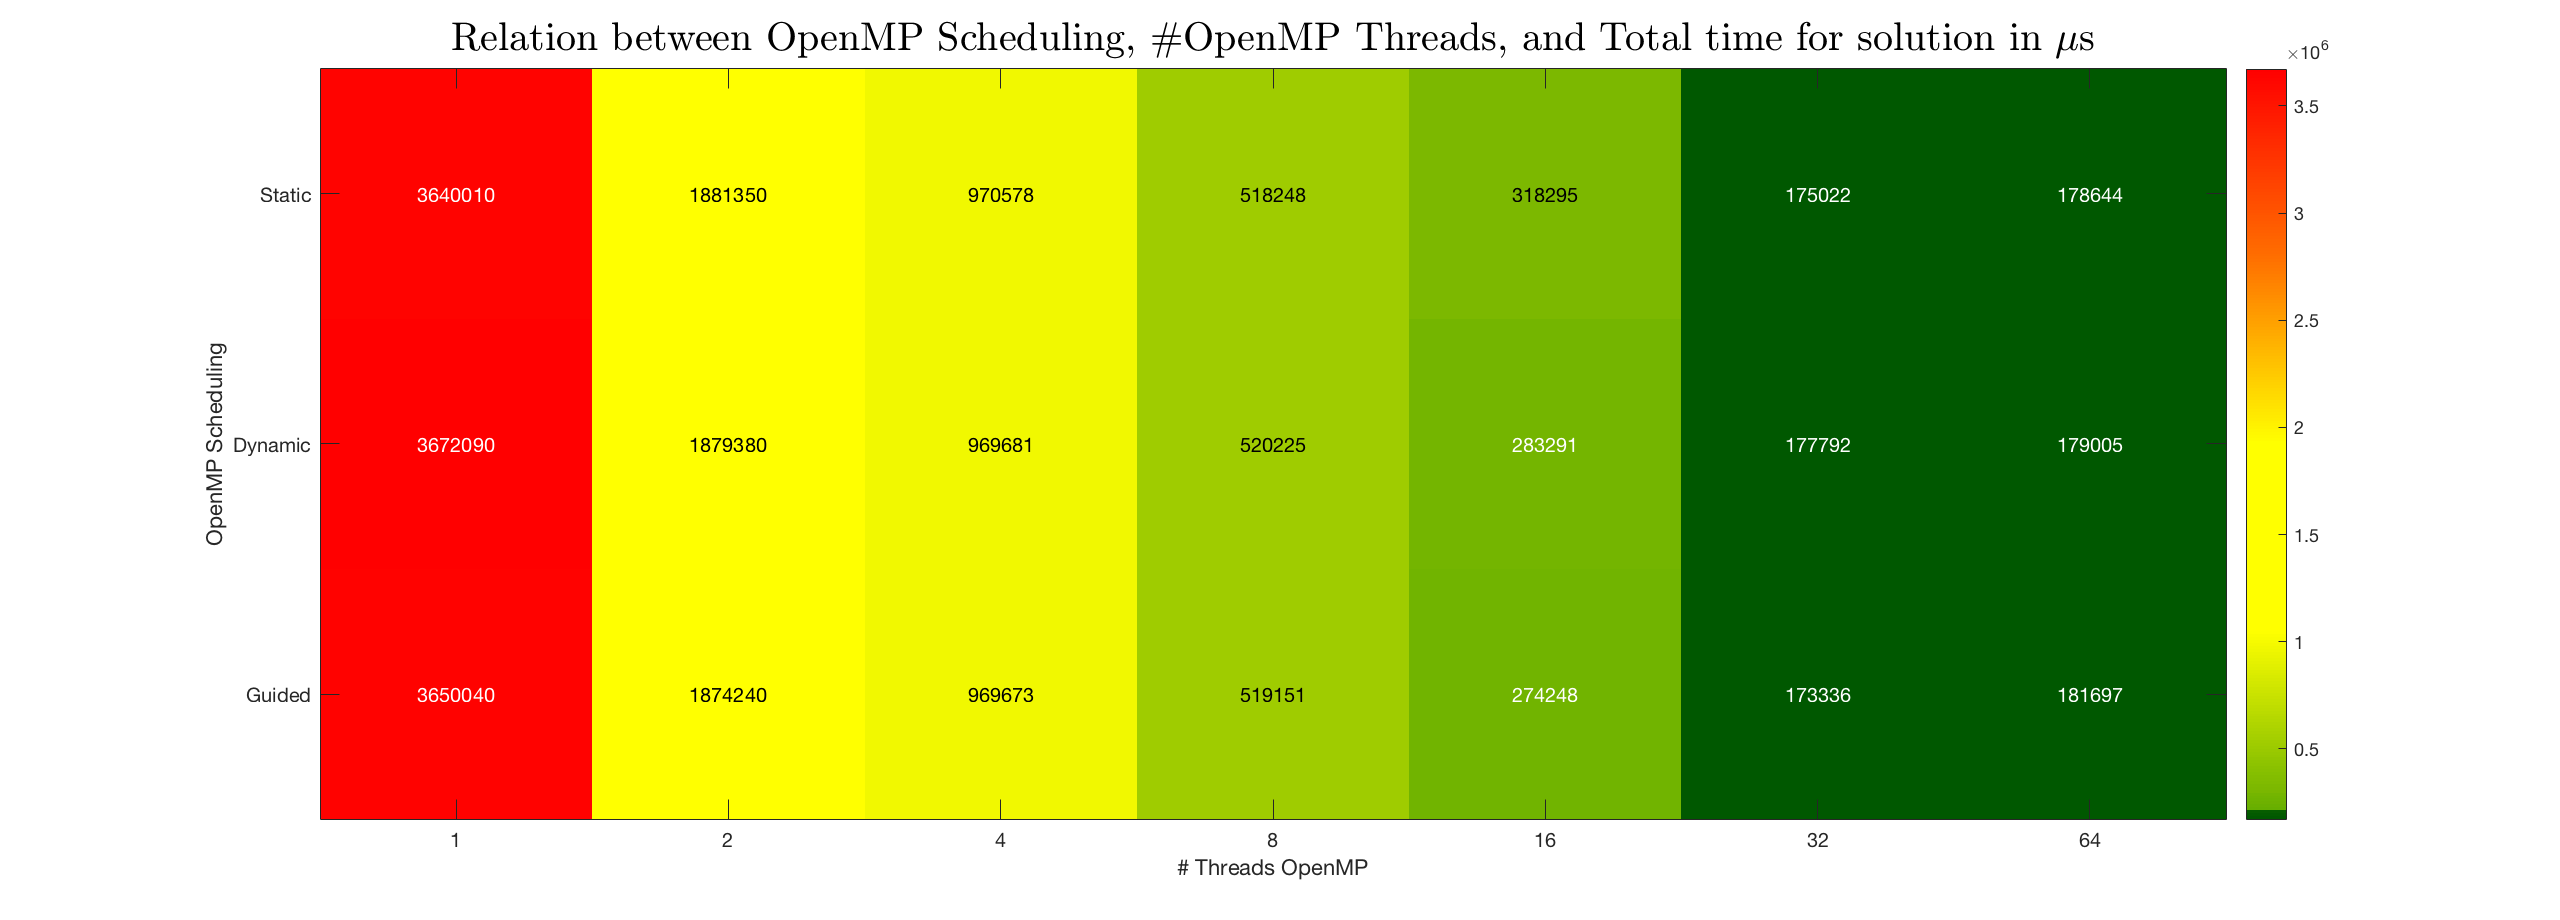
\includegraphics[width=1\columnwidth]{PNG/heatmap_scheduling_openmp_large.png}
\caption{ Relação entre o tipo de escalonamento OpenMP, número de Threads OpenMP, e tempo total para a solução, para uma gama de valores aleatórios do ciclo mais interior alterada ([1:262144]). }
\label{fig:heatmap_scheduling_openmp}
\end{figure}


Denote que com o aumento do número de iterações por thread, assim como da irregularidade de iterações por thread, dado o aumento da  gama de valores aleatórios do ciclo mais interior, resultou em dois comportamentos que merecem ser destacados. Se anteriormente tínhamos a melhor solução para o número de Threads igual a 1, neste momento é com 32 Threads OpenMP que se obtêm os melhores resultados. \par
Em adição podemos ainda verificar que apesar de apresentar um pouco ganho em comparação com o escalonamento \textbf{static}, o escalonamento \textbf{guided} foi o que apresentou melhores resultados. \par 
Para todos os números de Threads em teste, o escalonamento \textbf{dynamic} foi o que apresentou os resultados menos satisfatórios. Temos um problema que apesar de mais irregular quando comparado com o primeiro, ainda não toma partido das propriedades que tornam o escalonamento dinâmico uma mais valia.\par 

\label{tempos_exe3_gama_alterada}
Analisemos agora graficamente o comportamento das threads para o "worst-case-scenario" (1 Thread Dynamic) e "best-case-scenario" (32 Threads Guided) à semelhança do realizado anteriormente.
Desta forma, foram produzidas as figuras \ref{fig:best_large_guided_32_threads} a \ref{fig:worst_large_dynamic_1_threads}, ilustrando o descrito anteriormente.\par 


\subsubsection{Análise gráfica para o "best-case-scenario" dos tempos totais obtidos no estudo da secção \ref{tempos_exe3_gama_alterada}}

\begin{figure}[H]
\centering
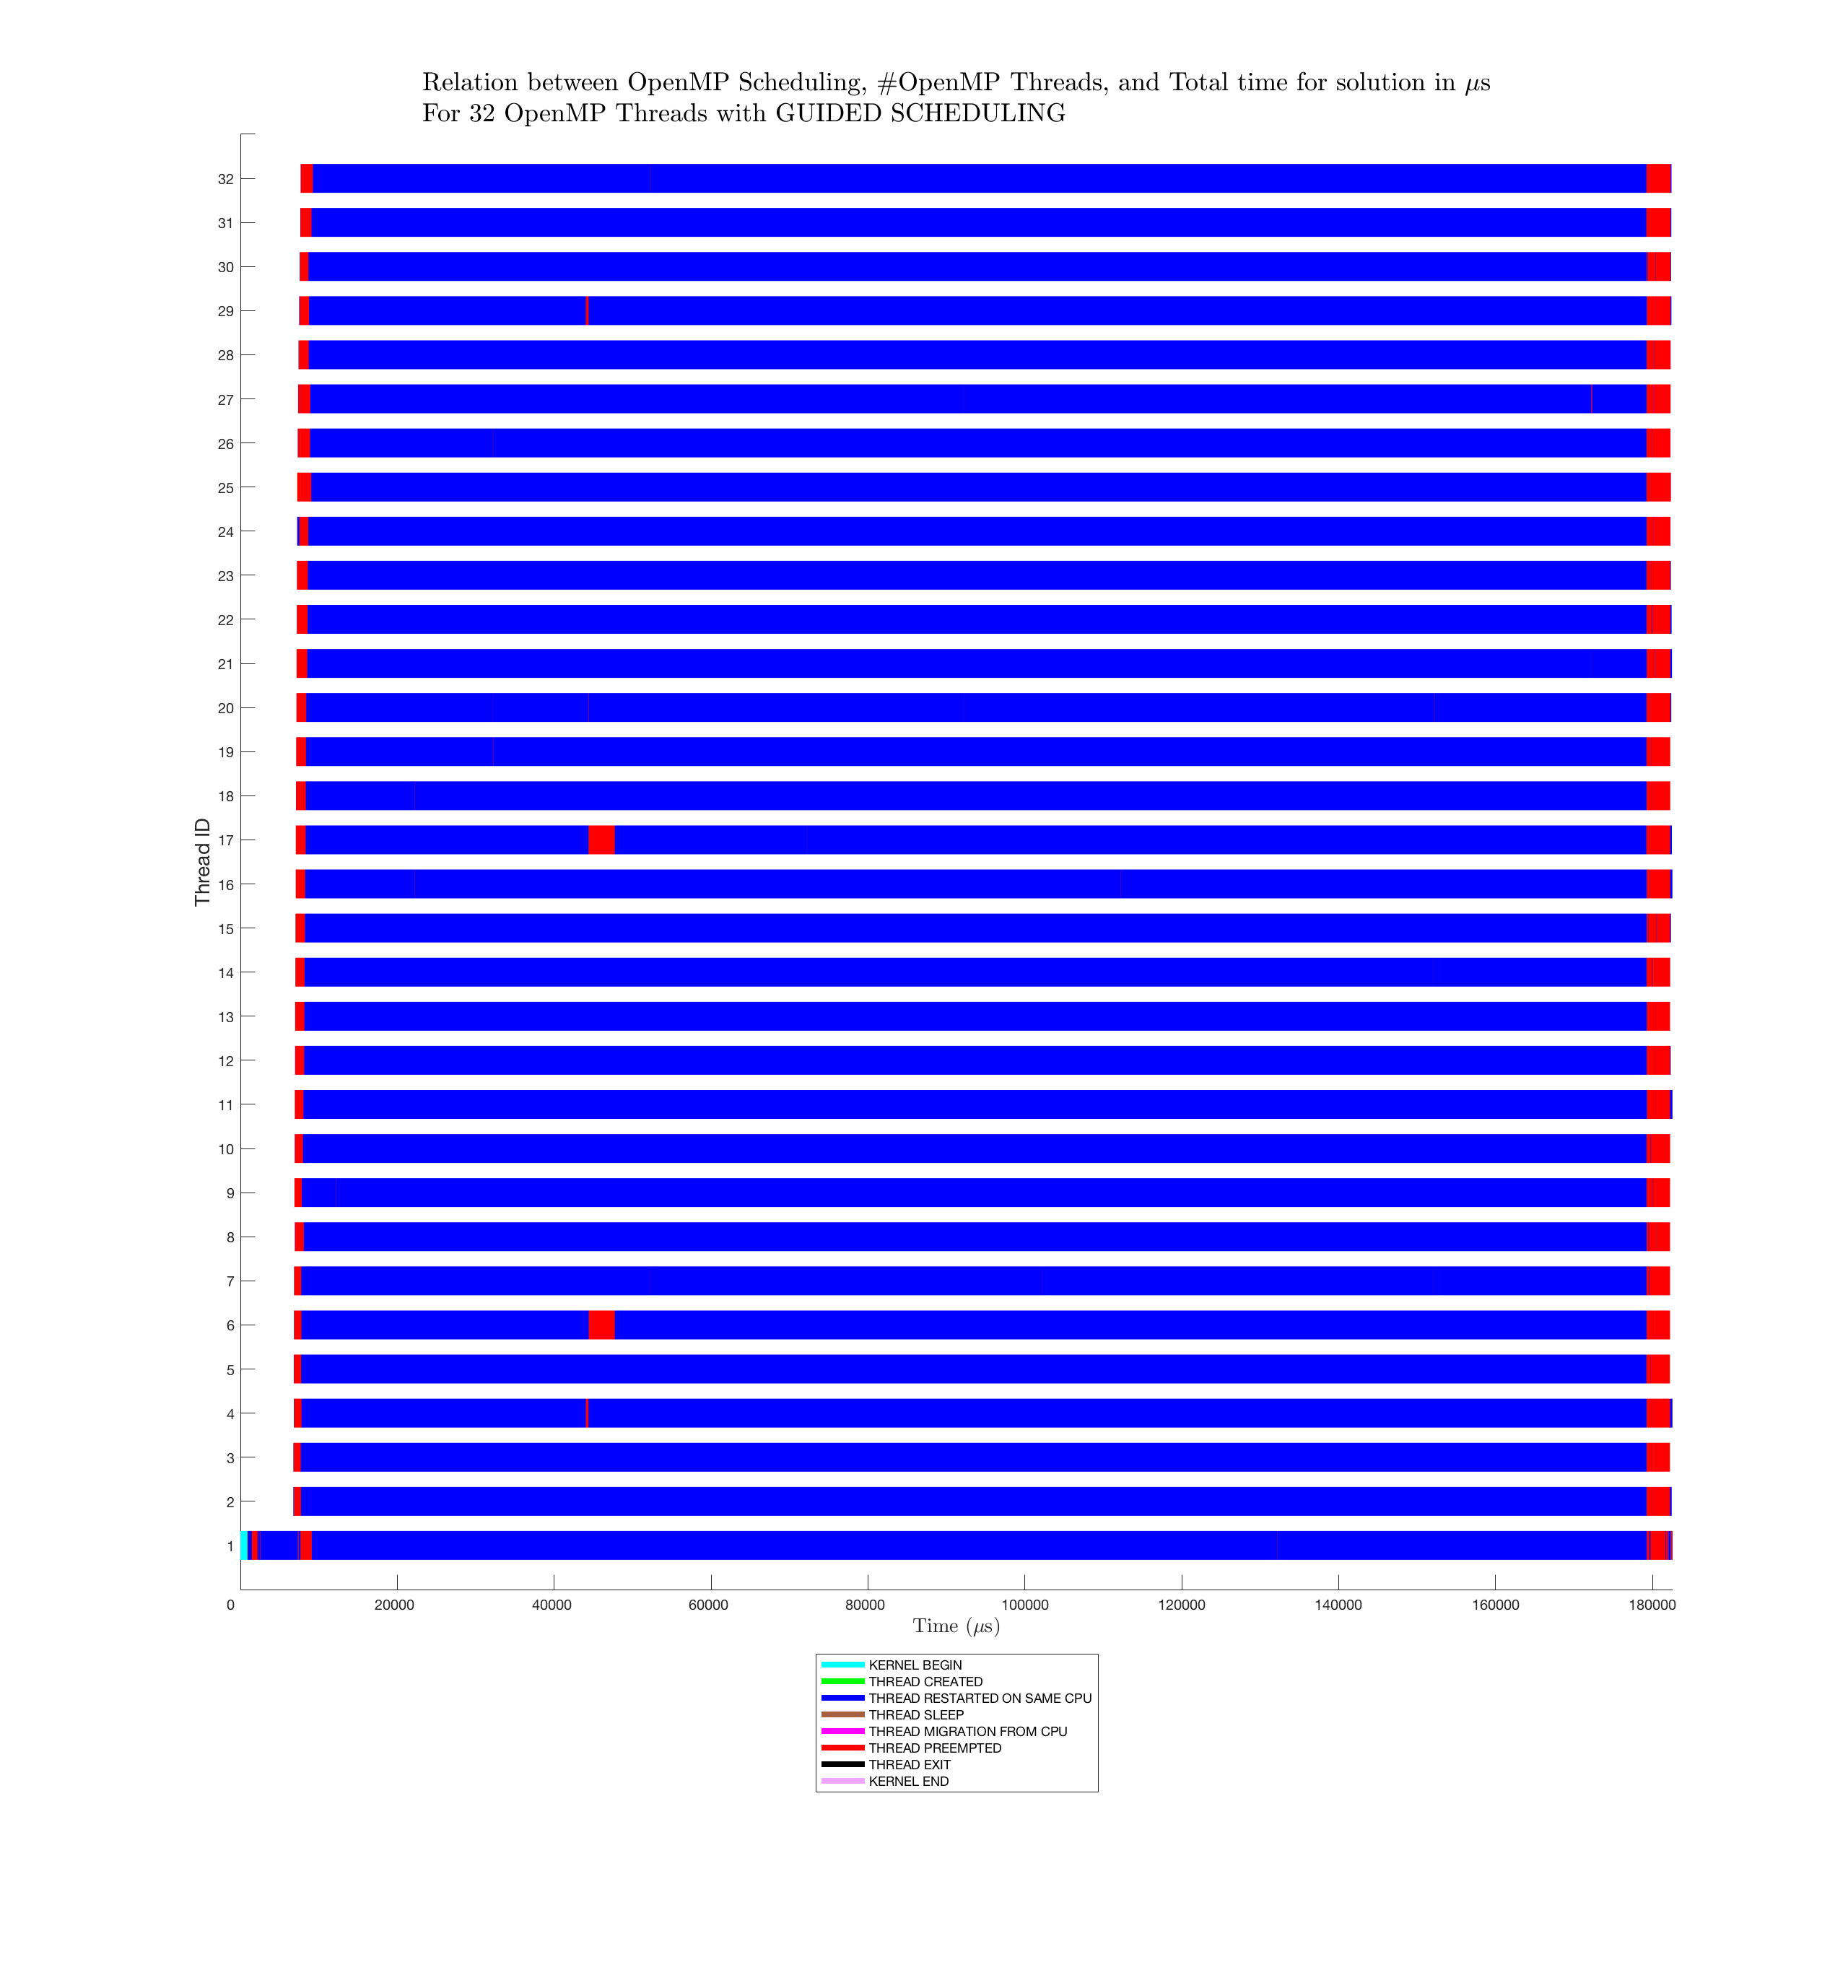
\includegraphics[width=0.9\columnwidth]{PNG/best_large_guided_32_threads.png}
\caption{ Análise gráfica para o "best-case-scenario" dos tempos totais obtidos no estudo da secção alterada ([1:262144]).  }
\label{fig:best_large_guided_32_threads}
\end{figure}


\subsubsection{Análise gráfica para o "worst-case-scenario" dos tempos totais obtidos no estudo da secção \ref{tempos_exe3_gama_alterada}}


\begin{figure}[H]
\centering
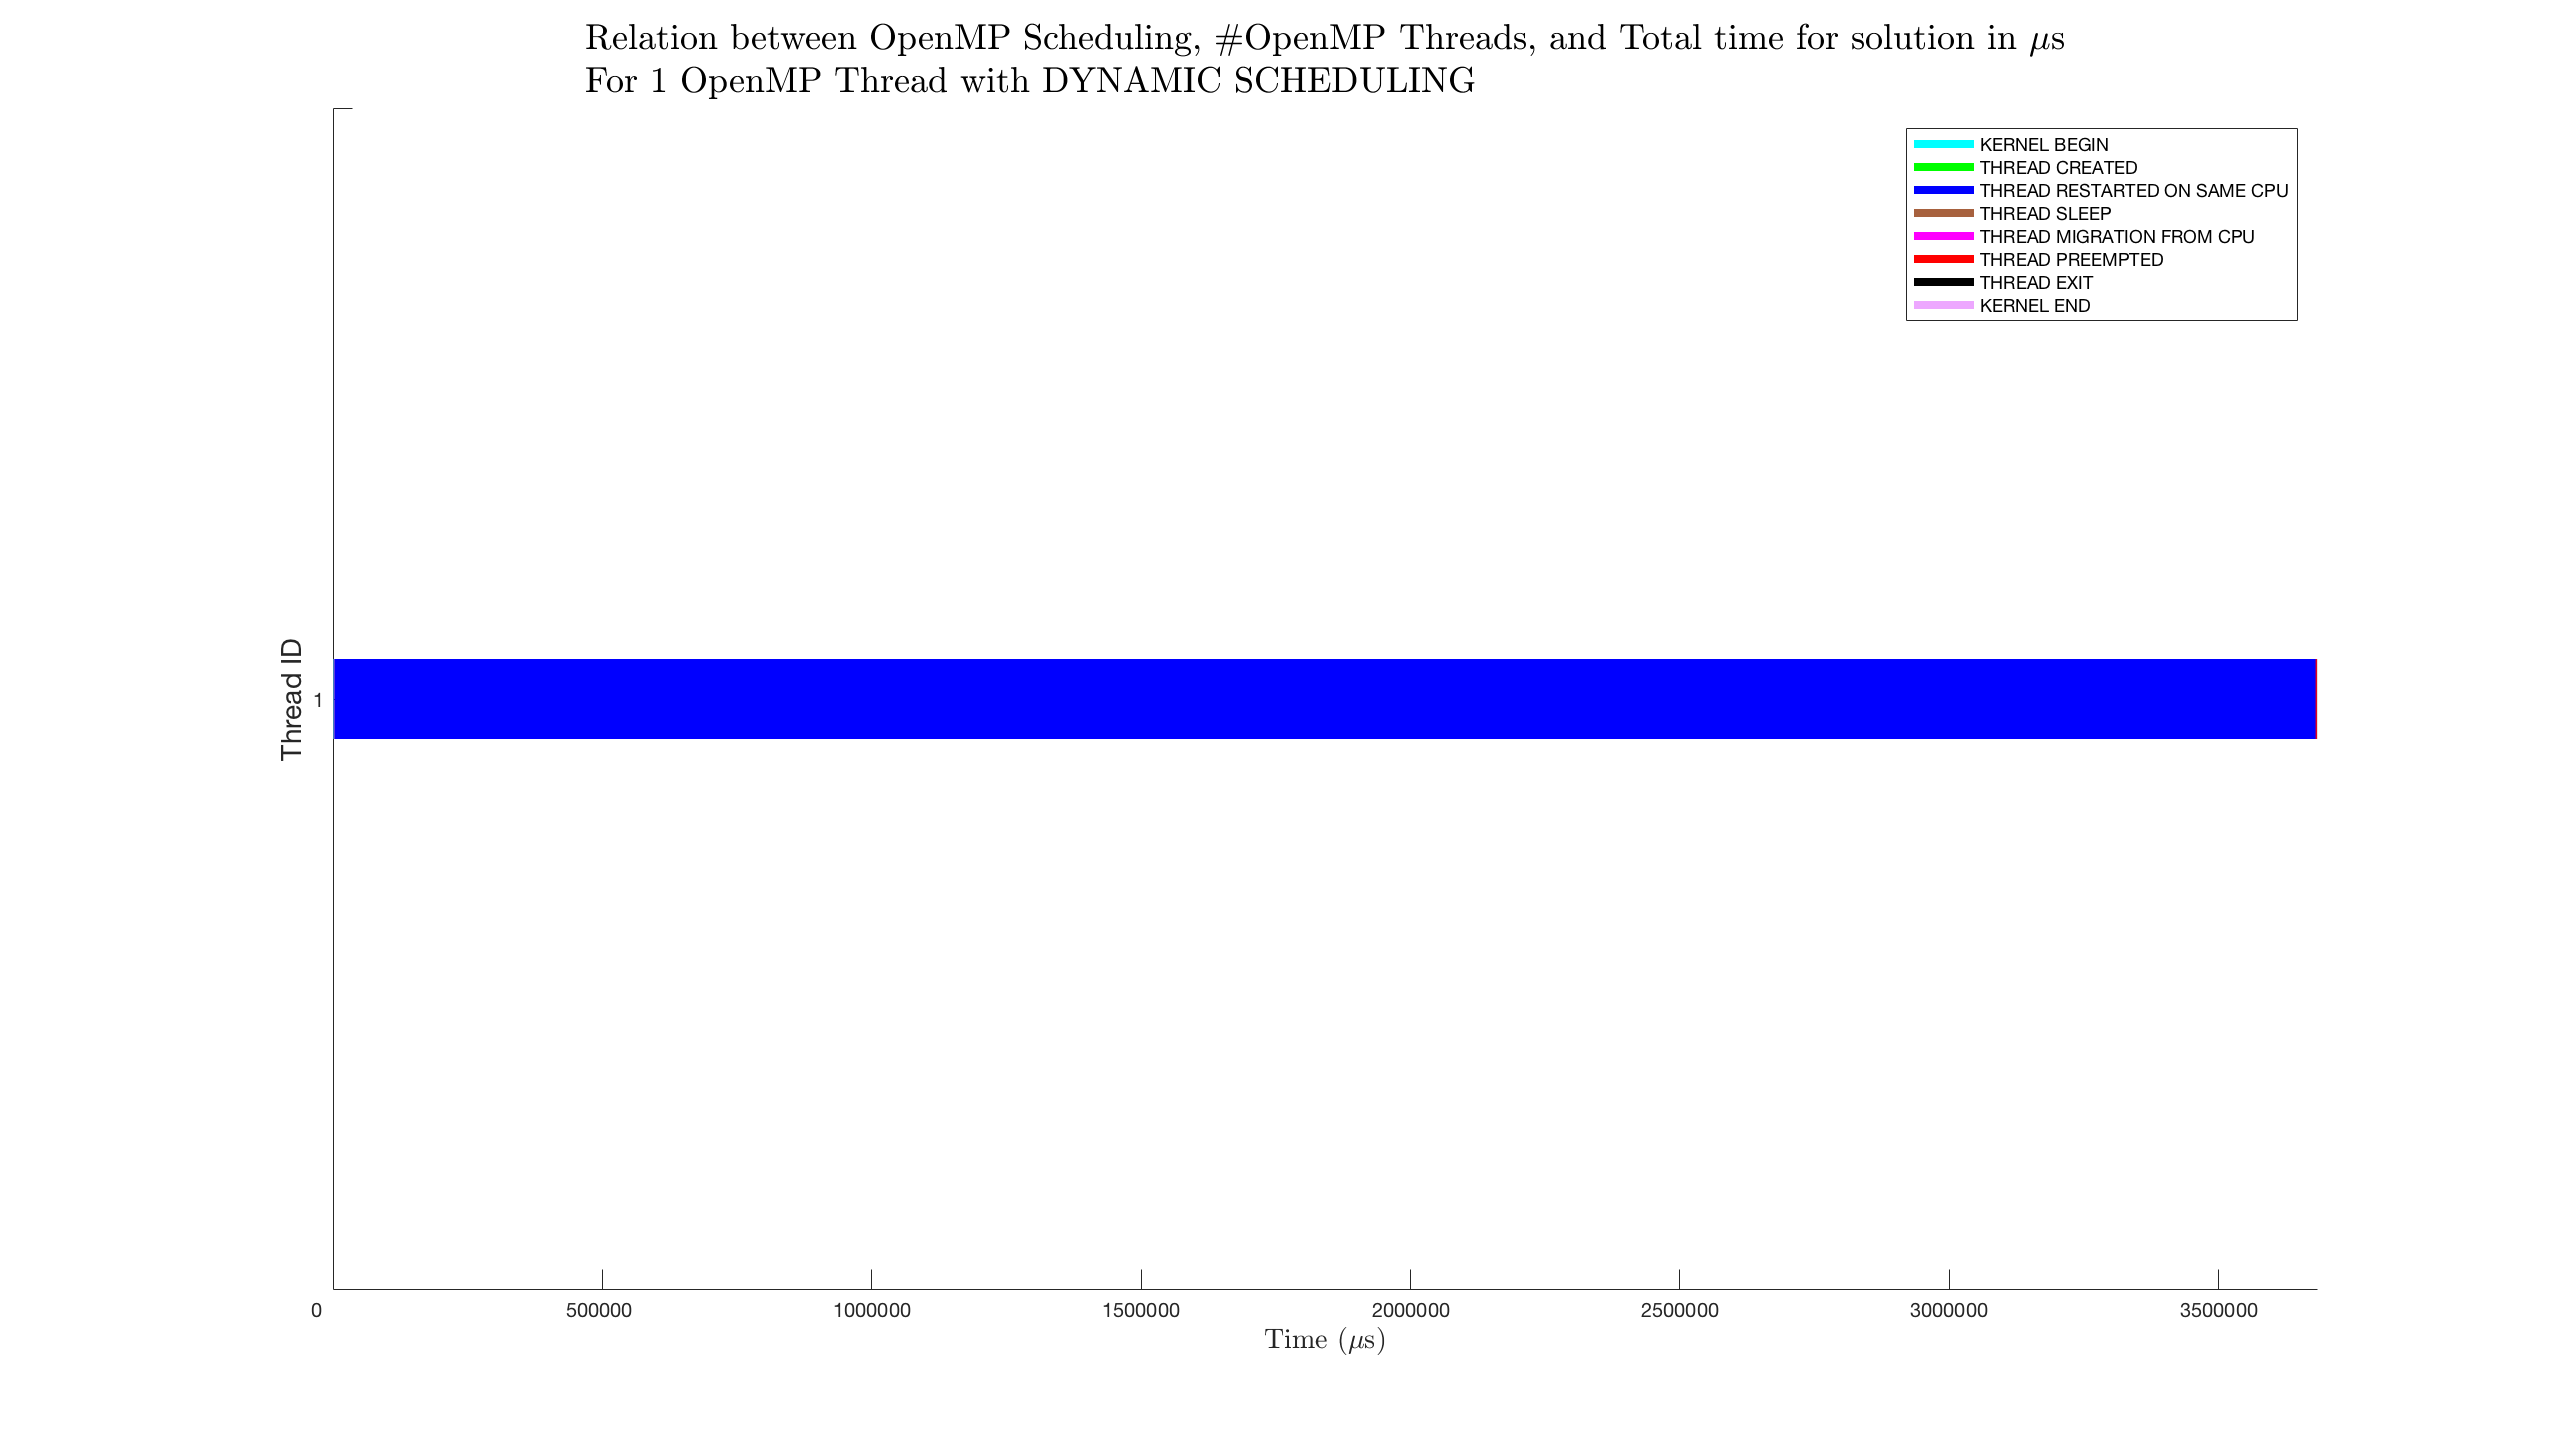
\includegraphics[width=0.9\columnwidth]{PNG/worst_large_dynamic_1_threads.png}
\caption{ Análise gráfica para o "worst-case-scenario" dos tempos totais obtidos no estudo da secção \ref{tempos_exe3_gama_alterada}, para uma gama de valores aleatórios do ciclo mais interior alterada  ([1:262144]).  }
\label{fig:worst_large_dynamic_1_threads}
\end{figure}

Ora, para ambos os escalonamentos aqui analisados, o tempo de CPU é aquele que a preserva esmagadora maioria de tempo -- padrão também verificado para para a gama de valores aleatórios. Atente apenas num pormenor na figura 
\ref{fig:best_large_guided_32_threads}. Para as threads 4 e 29, e 6 e 17, aquando da mudança de CPU das duas primeiras, dá-se um preempt das duas últimas, levando a concluir que as mesmas foram descalonadas, dando lugar às threads 4 e 29, passando as threads 6 e 17 a ocupar o lugar das anteriores.

\subsection{Conclusão do Trabalho Extra}

Através do exemplo anterior, é perfeitamente visível a granularidade com a qual podemos analisar os nossos kernels, permitindo uma possível correção de comportamentos que comprometam a performance dos mesmos. \par
Ora, o maior "problema" será mesmo definir qual a abordagem a tomar, dada a vasta gama de probes DTrace que permitem este tipo de análise. Mais importante para o trabalho de profiling que a ferramenta será a correcta identificação das métricas a medir -- sem essa compreensão nenhuma ferramenta poderá ajudar o programador.
\par 
Uma vez mais foi possível, de uma forma indirecta, desenvolver a prática em novos tipos de análise e tratamento de dados, assim como de bash scripting, pois dada extensão dos testes a realizar era necessária manter uma "estrutura" organizada sob pena de retirarmos conclusões erradas com base nos dados obtidos. Dessa mesma preocupação resultou o ficheiro final \textbf{threaded.d} de DTrace, que resultou da aplicação de conhecimento adquirido durante a Unidade Curricular ao ficheiro previamente fornecido na página da mesma.\par 


\end{document}


